\documentclass[aspectratio=169]{beamer}

\usetheme{default}
\usecolortheme{dove}
\setbeamertemplate{navigation symbols}{}
\setbeamertemplate{footline}{\hfill{\large\insertframenumber\,/\,\inserttotalframenumber}\hspace{1.8em}\vspace{0.5em}}

\usepackage{graphicx}
\usepackage{amsmath,amssymb}
\usepackage{tikz}
\usetikzlibrary{arrows.meta,positioning,calc,shapes.geometric}

\definecolor{popblue}{RGB}{52,101,164}
\definecolor{sampred}{RGB}{204,0,0}
\definecolor{paramgreen}{RGB}{0,140,70}
\definecolor{warnred}{RGB}{180,40,40}
\definecolor{orange1}{RGB}{220,120,0}
\definecolor{violet1}{RGB}{120,50,160}
\setbeamercolor{frametitle}{fg=popblue}
\setbeamercolor{title}{fg=popblue}

\newcommand{\source}[1]{\begin{tikzpicture}[remember picture,overlay]\node[anchor=south east,fill=black!70,text=white,inner sep=3pt,font=\scriptsize] at ([xshift=-0.25cm,yshift=0.18cm]current page.south east) {#1};\end{tikzpicture}}
\newcommand{\transition}[2]{\begin{frame}[plain]\vfill\begin{center}\color{popblue}\bfseries\fontsize{30}{34}\selectfont #1\par\vspace{0.7cm}\color{black}\Large #2\end{center}\vfill\end{frame}}

\title{Grokking and Mechanistic Interpretability}
\subtitle{How a tiny transformer learns modular addition with Fourier features}
\author{}
\date{}

\begin{document}

\begin{frame}
  \titlepage
  \vfill
  \small Power et al. (2022) \quad Nanda et al. (2023) \quad Welch Labs (2025)
\end{frame}

\begin{frame}
\frametitle{Roadmap}
\begin{enumerate}\setlength\itemsep{0.65em}
  \item The puzzle: why test performance can improve long after memorization.
  \item Generic transformer mechanics: how the $=$ position gathers and transforms information.
  \item The identified circuit: Fourier features make modular addition easy to express.
  \item Beyond the toy model: manifolds, superposition, and sparse autoencoders.
\end{enumerate}
\vfill
\begin{center}\fcolorbox{orange1}{orange1!10}{\parbox{0.82\linewidth}{\centering\large\textbf{Running example:} $P=7$, so the prompt $2\quad3\quad=$ should produce $5$.}}\end{center}
\end{frame}

% ----------------------------------------------------------------
\section{The puzzle}
\transition{The puzzle}{A model can memorize first and understand later.}

\begin{frame}
\frametitle{Predict first: is training accuracy the whole story?}
\begin{center}
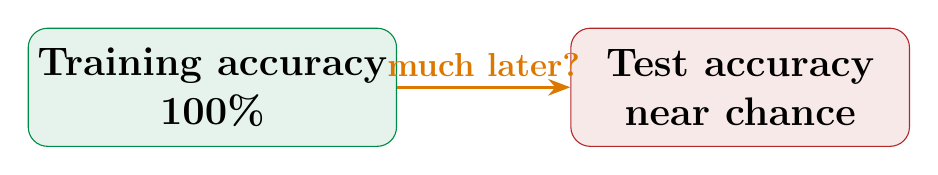
\begin{tikzpicture}[node distance=1.2cm and 2.2cm]
\node[draw=paramgreen,fill=paramgreen!10,rounded corners=7pt,minimum width=4.3cm,minimum height=1.5cm,align=center,font=\Large\bfseries] (train) {Training accuracy\\100\%};
\node[draw=warnred,fill=warnred!10,rounded corners=7pt,minimum width=4.3cm,minimum height=1.5cm,align=center,font=\Large\bfseries,right=of train] (test) {Test accuracy\\near chance};
\draw[-{Stealth[length=8pt]},very thick,orange1] (train) -- (test) node[midway,above,font=\large\bfseries] {much later?};
\end{tikzpicture}
\end{center}
\vspace{0.7cm}
\begin{center}\Large\color{popblue}\textbf{Grokking:} delayed generalization after apparent overfitting.\end{center}
\end{frame}

\begin{frame}
\frametitle{The task: fill in an incomplete modular-addition table}
\begin{columns}[T]
\column{0.52\textwidth}
\begin{itemize}\setlength\itemsep{0.5em}
  \item Work modulo $P$: after $P-1$, wrap back to $0$.
  \item Running example with $P=7$: $2+3=5\pmod 7$.
  \item Train on a random subset of pairs $(a,b)$.
  \item Test on the missing cells of the table.
\end{itemize}
\column{0.48\textwidth}
\begin{center}
\begin{tabular}{c|rrrrrrr}
$+$ mod 7&0&1&2&3&4&5&6\\\hline
0&0&1&2&3&4&5&6\\
1&1&2&3&4&5&6&0\\
2&2&3&4&5&6&0&1\\
3&3&4&5&6&0&1&2\\
4&4&5&6&0&1&2&3
\end{tabular}
\end{center}
\end{columns}
\end{frame}

{
\usebackgroundtemplate{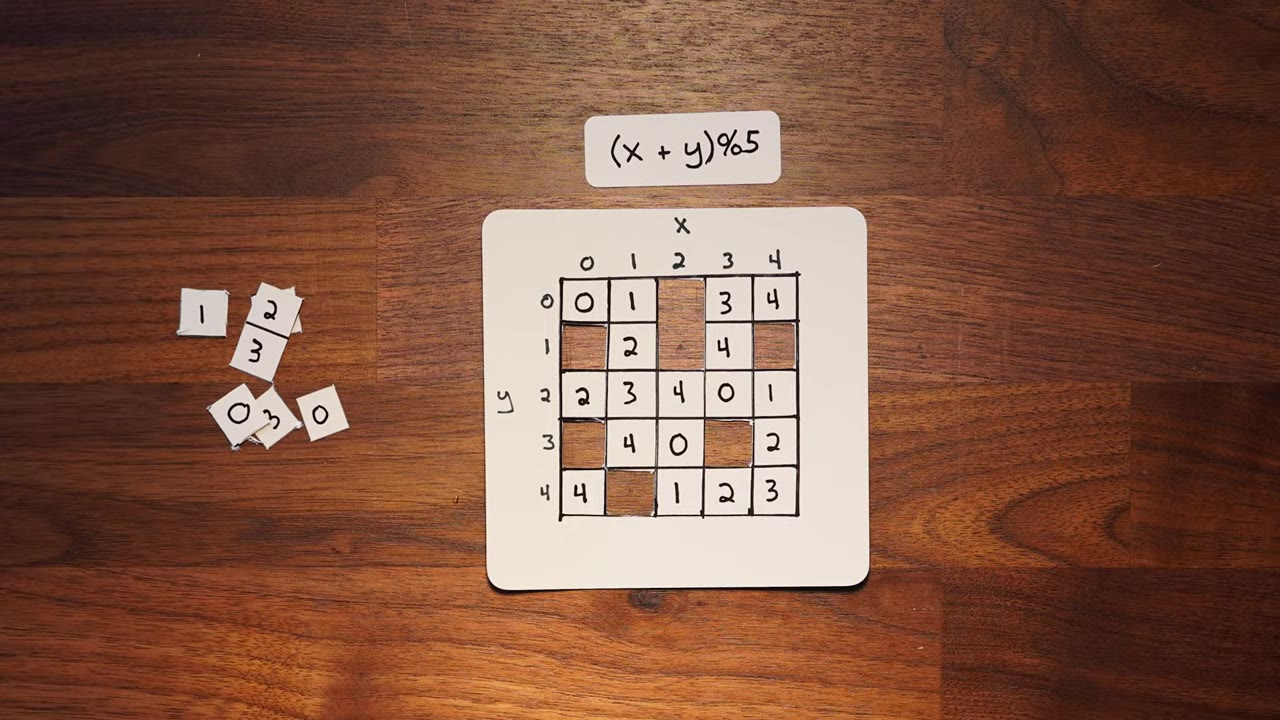
\includegraphics[width=\paperwidth,height=\paperheight]{../frames/f01_00-03-52.jpg}}
\begin{frame}[plain]
\source{Welch Labs, modular-addition table, 03:52}
\end{frame}
}

\begin{frame}
\frametitle{What the classic grokking curve means}
\begin{center}
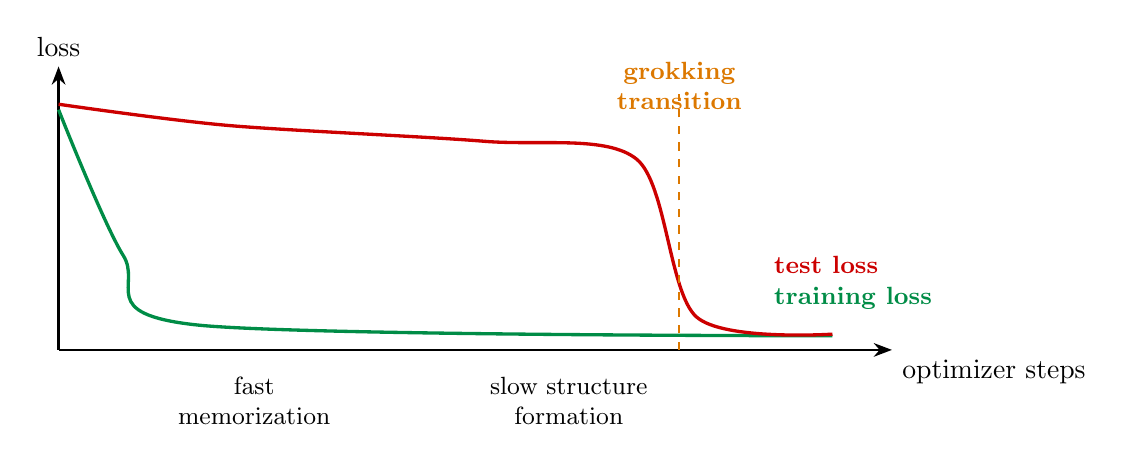
\begin{tikzpicture}[x=2.16cm,y=1.0cm]
\draw[-{Stealth},thick] (0,0)--(4.9,0) node[below right]{optimizer steps};
\draw[-{Stealth},thick] (0,0)--(0,3.6) node[above]{loss};
\draw[paramgreen,very thick] plot[smooth] coordinates {(0,3.05)(.38,1.2)(.8,.32)(4.55,.18)};
\draw[sampred,very thick] plot[smooth] coordinates {(0,3.12)(1.0,2.85)(2.5,2.65)(3.4,2.42)(3.75,.42)(4.55,.2)};
\draw[dashed,orange1,thick] (3.65,0)--(3.65,3.25);
\node[paramgreen,font=\small\bfseries,anchor=west] at (4.15,.65) {training loss};
\node[sampred,font=\small\bfseries,anchor=west] at (4.15,1.08) {test loss};
\node[orange1,font=\small\bfseries,align=center] at (3.65,3.35) {grokking\\transition};
\node[font=\small,align=center] at (1.15,-.65) {fast\\memorization};
\node[font=\small,align=center] at (3.0,-.65) {slow structure\\formation};
\end{tikzpicture}
\end{center}
\vfill
\small This is a conceptual learning curve: the point is the gap between fast fitting and late held-out improvement.
\end{frame}

{
\usebackgroundtemplate{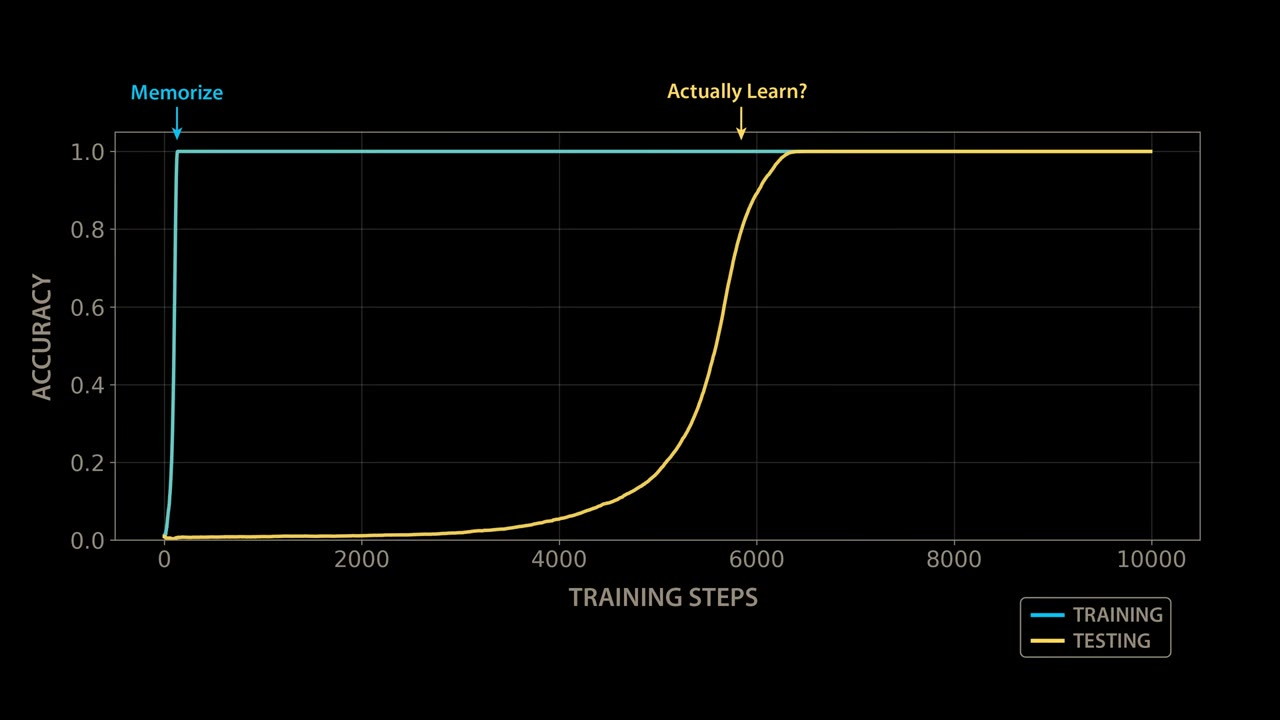
\includegraphics[width=\paperwidth,height=\paperheight]{../frames/f02_00-07-56.jpg}}
\begin{frame}[plain]
\source{Welch Labs, grokking learning curve, 07:56}
\end{frame}
}

% ----------------------------------------------------------------
\section{Inside this transformer}
\transition{Generic transformer mechanics}{Follow $2\quad3\quad=$ from symbols to a prediction. The next section identifies the particular circuit this model learns.}

\begin{frame}
\frametitle{The whole computation, at one glance}
\begin{center}
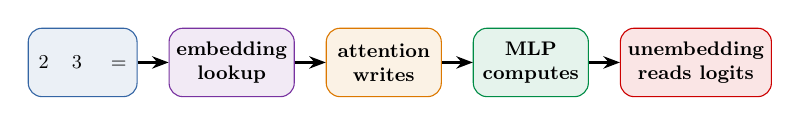
\begin{tikzpicture}[node distance=0.58cm and 0.50cm,scale=.79,transform shape]
\node[draw=popblue,fill=popblue!10,rounded corners=5pt,minimum width=1.75cm,minimum height=1.1cm,align=center,font=\small\bfseries] (input) {$2\quad 3\quad =$};
\node[draw=violet1,fill=violet1!10,rounded corners=5pt,minimum width=1.85cm,minimum height=1.1cm,align=center,font=\small\bfseries,right=of input] (embed) {embedding\\lookup};
\node[draw=orange1,fill=orange1!10,rounded corners=5pt,minimum width=1.85cm,minimum height=1.1cm,align=center,font=\small\bfseries,right=of embed] (attn) {attention\\writes};
\node[draw=paramgreen,fill=paramgreen!10,rounded corners=5pt,minimum width=1.85cm,minimum height=1.1cm,align=center,font=\small\bfseries,right=of attn] (mlp) {MLP\\computes};
\node[draw=sampred,fill=sampred!10,rounded corners=5pt,minimum width=1.85cm,minimum height=1.1cm,align=center,font=\small\bfseries,right=of mlp] (out) {unembedding\\reads logits};
\foreach \a/\b in {input/embed,embed/attn,attn/mlp,mlp/out} \draw[-{Stealth[length=6pt]},thick] (\a)--(\b);
\end{tikzpicture}
\end{center}
\vspace{0.45cm}
\begin{block}{The special output position}
For our running input $2\quad3\quad=$, the model reads the residual stream at $=$ and should assign the largest logit to $c=5$.
\end{block}
\end{frame}

\begin{frame}
\frametitle{Step 1: tokens become vectors}
\begin{columns}[c]
\column{0.50\textwidth}
\begin{itemize}\setlength\itemsep{0.55em}
\item The vocabulary contains the residues and symbols such as $=$.
\item A learned table maps each token to a vector: $e(n),e(=)\in\mathbb{R}^{d_{\mathrm{model}}}$.
\item For the running prompt, lookup produces $e(2),e(3),e(=)$.
\item At this stage, token IDs are just labels. No addition rule is built in.
\end{itemize}
\column{0.50\textwidth}
\begin{center}
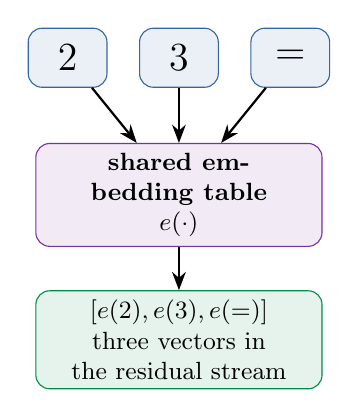
\begin{tikzpicture}[node distance=.4cm]
\node[draw=popblue,fill=popblue!10,rounded corners=5pt,minimum width=1.0cm,minimum height=.75cm,font=\Large] (a) {$2$};
\node[draw=popblue,fill=popblue!10,rounded corners=5pt,minimum width=1.0cm,minimum height=.75cm,right=of a,font=\Large] (b) {$3$};
\node[draw=popblue,fill=popblue!10,rounded corners=5pt,minimum width=1.0cm,minimum height=.75cm,right=of b,font=\Large] (eq) {$=$};
\node[draw=violet1,fill=violet1!10,rounded corners=5pt,text width=3.4cm,minimum height=1.0cm,align=center,below=.7cm of b,font=\small\bfseries] (table) {shared embedding table\\$e(\cdot)$};
\draw[-{Stealth},thick] (a)--(table);
\draw[-{Stealth},thick] (b)--(table);
\draw[-{Stealth},thick] (eq)--(table);
\node[draw=paramgreen,fill=paramgreen!10,rounded corners=5pt,text width=3.4cm,minimum height=1.0cm,align=center,below=.55cm of table,font=\small] (vectors) {$[e(2),e(3),e(=)]$\\three vectors in the residual stream};
\draw[-{Stealth},thick] (table)--(vectors);
\end{tikzpicture}
\end{center}
\end{columns}
\end{frame}

\begin{frame}
\frametitle{Step 2: position says which role each token plays}
\begin{center}
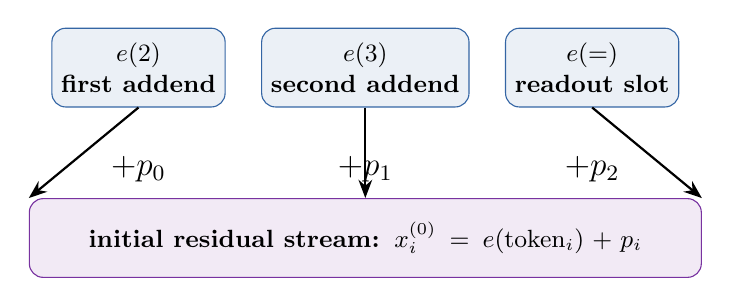
\begin{tikzpicture}[node distance=.85cm and .45cm]
\node[draw=popblue,fill=popblue!10,rounded corners=5pt,minimum width=2.15cm,minimum height=1.0cm,align=center,font=\small\bfseries] (ea) {$e(2)$\\first addend};
\node[draw=popblue,fill=popblue!10,rounded corners=5pt,minimum width=2.15cm,minimum height=1.0cm,align=center,font=\small\bfseries,right=of ea] (eb) {$e(3)$\\second addend};
\node[draw=popblue,fill=popblue!10,rounded corners=5pt,minimum width=2.15cm,minimum height=1.0cm,align=center,font=\small\bfseries,right=of eb] (eeq) {$e(=)$\\readout slot};
\node[below=.5cm of ea,font=\large] {$+p_0$};
\node[below=.5cm of eb,font=\large] {$+p_1$};
\node[below=.5cm of eeq,font=\large] {$+p_2$};
\node[draw=violet1,fill=violet1!10,rounded corners=5pt,text width=8.3cm,minimum height=1.0cm,align=center,below=1.15cm of eb,font=\small\bfseries] (stream) {initial residual stream: $x_i^{(0)}=e(\mathrm{token}_i)+p_i$};
\draw[-{Stealth},thick] (ea.south)--(stream.north west);
\draw[-{Stealth},thick] (eb.south)--(stream.north);
\draw[-{Stealth},thick] (eeq.south)--(stream.north east);
\end{tikzpicture}
\end{center}
\vfill
\small Position vectors matter because $2$, $3$, and $=$ must receive different computational roles even when all are tokens.
\end{frame}

\begin{frame}
\frametitle{The residual stream is the model's shared workspace}
\begin{columns}[c]
\column{0.52\textwidth}
\begin{itemize}\setlength\itemsep{0.55em}
\item Every layer reads the current vector at each position.
\item Attention and the MLP each write an update back into the same space.
\item The additions are literal: $x\leftarrow x+\Delta_{\mathrm{attn}}+\Delta_{\mathrm{MLP}}$.
\item Mechanistic interpretability tracks what each update adds to the answer position.
\end{itemize}
\column{0.48\textwidth}
\begin{center}
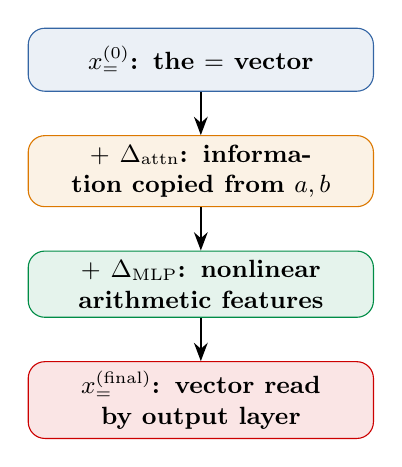
\begin{tikzpicture}[node distance=.55cm]
\node[draw=popblue,fill=popblue!10,rounded corners=6pt,text width=4.15cm,minimum height=.8cm,align=center,font=\small\bfseries] (x0) {$x_{=}^{(0)}$: the $=$ vector};
\node[draw=orange1,fill=orange1!10,rounded corners=6pt,text width=4.15cm,minimum height=.8cm,align=center,font=\small\bfseries,below=of x0] (attn) {$+\ \Delta_{\mathrm{attn}}$: information copied from $a,b$};
\node[draw=paramgreen,fill=paramgreen!10,rounded corners=6pt,text width=4.15cm,minimum height=.8cm,align=center,font=\small\bfseries,below=of attn] (mlp) {$+\ \Delta_{\mathrm{MLP}}$: nonlinear arithmetic features};
\node[draw=sampred,fill=sampred!10,rounded corners=6pt,text width=4.15cm,minimum height=.8cm,align=center,font=\small\bfseries,below=of mlp] (final) {$x_{=}^{(\mathrm{final})}$: vector read by output layer};
\draw[-{Stealth},thick] (x0)--(attn);
\draw[-{Stealth},thick] (attn)--(mlp);
\draw[-{Stealth},thick] (mlp)--(final);
\end{tikzpicture}
\end{center}
\end{columns}
\end{frame}

{
\usebackgroundtemplate{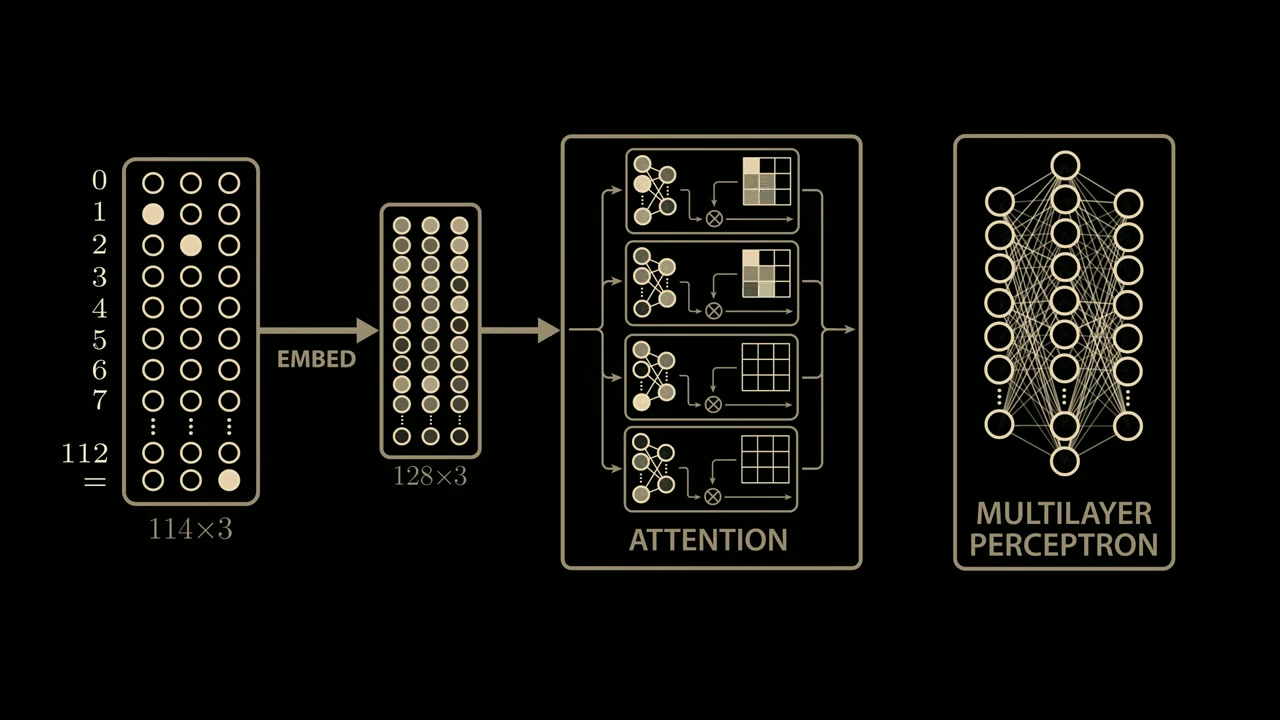
\includegraphics[width=\paperwidth,height=\paperheight]{../frames/f14_00-10-20.jpg}}
\begin{frame}[plain]
\source{Welch Labs, attention and residual stream, 10:20}
\end{frame}
}

\begin{frame}
\frametitle{Step 3: attention routes $2$ and $3$ into the equals position}
\begin{center}
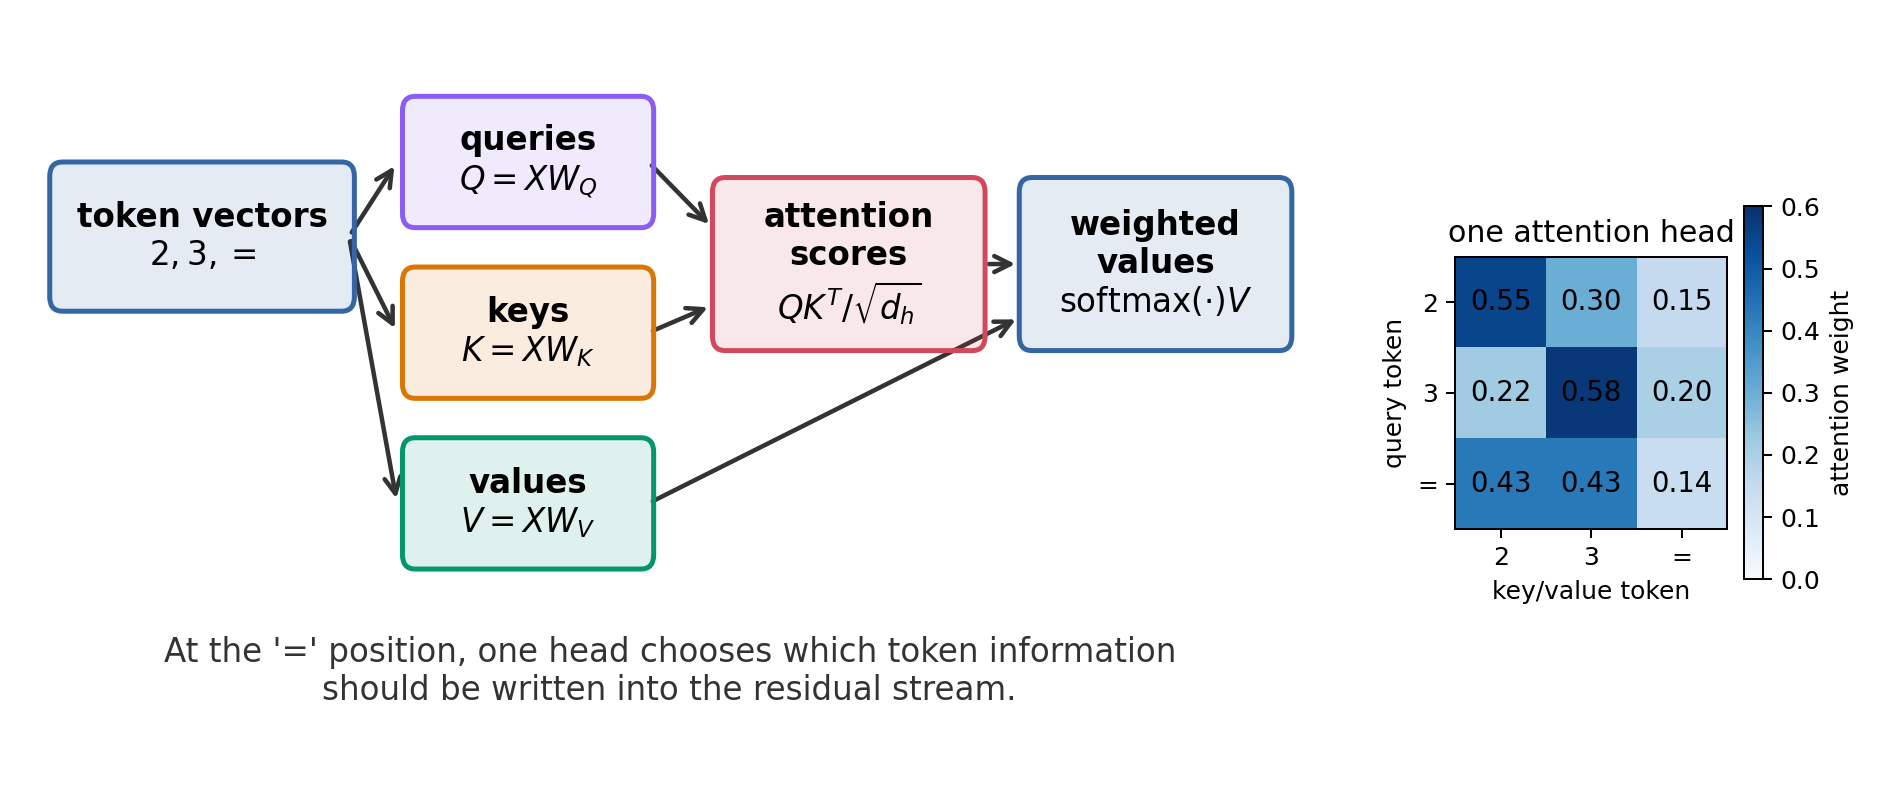
\includegraphics[width=.96\textwidth,height=.68\textheight,keepaspectratio]{fig/attention_mechanics.png}
\end{center}
\vfill
\small In this generic schematic, only the query at $=$ matters: it should fetch both operand vectors into one workspace.
\end{frame}

\begin{frame}
\frametitle{Attention is a data-dependent weighted sum}
\begin{columns}[T]
\column{0.54\textwidth}
\[
Q=XW_Q,\qquad K=XW_K,\qquad V=XW_V
\]
\[
A=\mathrm{softmax}\left(\frac{QK^\top}{\sqrt{d_h}}\right)
\qquad
\Delta_{\mathrm{attn}}=AVW_O
\]
\begin{itemize}\setlength\itemsep{0.35em}
\item Row $A_{=,:}$ determines what the $=$ position reads.
\item Large weights on $2$ and $3$ route both addends into one workspace.
\item $W_O$ returns each head's result to the residual stream.
\end{itemize}
\column{0.46\textwidth}
\begin{center}
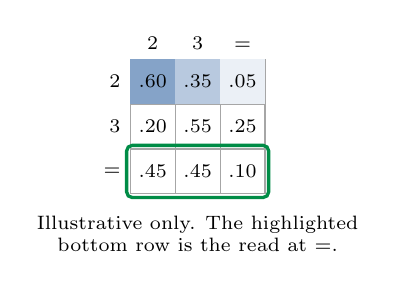
\begin{tikzpicture}[scale=.92]
\draw[step=.62cm,black!35] (0,0) grid (1.86,1.86);
\fill[popblue!60] (0,1.24) rectangle (.62,1.86);
\fill[popblue!35] (.62,1.24) rectangle (1.24,1.86);
\fill[popblue!10] (1.24,1.24) rectangle (1.86,1.86);
\node[font=\scriptsize] at (.31,1.55) {.60};
\node[font=\scriptsize] at (.93,1.55) {.35};
\node[font=\scriptsize] at (1.55,1.55) {.05};
\node[font=\scriptsize] at (.31,.93) {.20};
\node[font=\scriptsize] at (.93,.93) {.55};
\node[font=\scriptsize] at (1.55,.93) {.25};
\node[font=\scriptsize] at (.31,.31) {.45};
\node[font=\scriptsize] at (.93,.31) {.45};
\node[font=\scriptsize] at (1.55,.31) {.10};
\node[font=\scriptsize,above] at (.31,1.86) {$2$};
\node[font=\scriptsize,above] at (.93,1.86) {$3$};
\node[font=\scriptsize,above] at (1.55,1.86) {$=$};
\node[font=\scriptsize,left] at (0,1.55) {$2$};
\node[font=\scriptsize,left] at (0,.93) {$3$};
\node[font=\scriptsize,left] at (0,.31) {$=$};
\draw[paramgreen,very thick,rounded corners=2pt] (-.05,-.05) rectangle (1.91,.67);
\node[font=\scriptsize,align=center] at (.93,-.55) {Illustrative only. The highlighted\\bottom row is the read at $=$.};
\end{tikzpicture}
\end{center}
\end{columns}
\end{frame}

\begin{frame}
\frametitle{Multiple heads are parallel communication channels}
\begin{center}
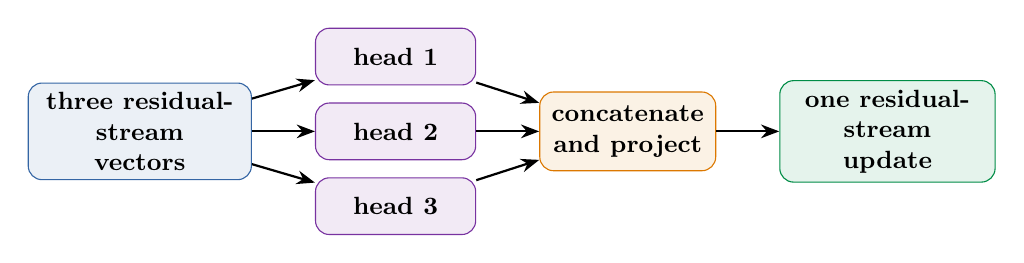
\begin{tikzpicture}[node distance=.7cm and .8cm]
\node[draw=popblue,fill=popblue!10,rounded corners=5pt,text width=2.6cm,minimum height=1.0cm,align=center,font=\small\bfseries] (stream) {three residual-stream\\vectors};
\node[draw=violet1,fill=violet1!10,rounded corners=5pt,text width=1.8cm,minimum height=.72cm,align=center,font=\small\bfseries,right=of stream,yshift=.95cm] (h1) {head 1};
\node[draw=violet1,fill=violet1!10,rounded corners=5pt,text width=1.8cm,minimum height=.72cm,align=center,font=\small\bfseries,right=of stream] (h2) {head 2};
\node[draw=violet1,fill=violet1!10,rounded corners=5pt,text width=1.8cm,minimum height=.72cm,align=center,font=\small\bfseries,right=of stream,yshift=-.95cm] (h3) {head 3};
\node[draw=orange1,fill=orange1!10,rounded corners=5pt,text width=2.0cm,minimum height=1.0cm,align=center,font=\small\bfseries,right=of h2] (concat) {concatenate\\and project};
\node[draw=paramgreen,fill=paramgreen!10,rounded corners=5pt,text width=2.5cm,minimum height=1.0cm,align=center,font=\small\bfseries,right=of concat] (write) {one residual-stream\\update};
\foreach \h in {h1,h2,h3}{\draw[-{Stealth},thick] (stream)--(\h);}
\foreach \h in {h1,h2,h3}{\draw[-{Stealth},thick] (\h)--(concat);}
\draw[-{Stealth},thick] (concat)--(write);
\end{tikzpicture}
\end{center}
\vspace{.45cm}
\small A small modular-addition model is much simpler than a modern language model, but the same Q/K/V communication pattern is present.
\end{frame}

\begin{frame}
\frametitle{Step 4: the MLP makes nonlinear features}
\begin{columns}[c]
\column{0.52\textwidth}
\small
\[
h=\mathrm{ReLU}(W_{\mathrm{in}}x+b_{\mathrm{in}}),
\quad
\Delta_{\mathrm{MLP}}=W_{\mathrm{out}}h+b_{\mathrm{out}}
\]
\normalsize
\begin{itemize}\setlength\itemsep{0.45em}
\item Each hidden neuron is a learned detector on the current residual vector.
\item ReLU gates that detector on or off.
\item A weighted sum of many hidden units can approximate nonlinear functions of the two inputs.
\item Here, the useful nonlinear evidence should support the candidate answer $5$.
\end{itemize}
\column{0.48\textwidth}
\begin{center}
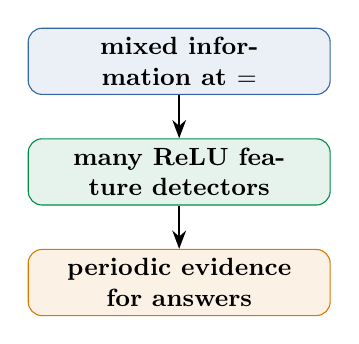
\begin{tikzpicture}[node distance=.55cm]
\node[draw=popblue,fill=popblue!10,rounded corners=5pt,text width=3.6cm,minimum height=.8cm,align=center,font=\small\bfseries] (in) {mixed information at $=$};
\node[draw=paramgreen,fill=paramgreen!10,rounded corners=5pt,text width=3.6cm,minimum height=.8cm,align=center,font=\small\bfseries,below=of in] (hidden) {many ReLU feature detectors};
\node[draw=orange1,fill=orange1!10,rounded corners=5pt,text width=3.6cm,minimum height=.8cm,align=center,font=\small\bfseries,below=of hidden] (out) {periodic evidence for answers};
\draw[-{Stealth},thick] (in)--(hidden);
\draw[-{Stealth},thick] (hidden)--(out);
\end{tikzpicture}
\end{center}
\end{columns}
\end{frame}

\begin{frame}
\frametitle{The MLP converts periodic input features into answer evidence}
\begin{center}
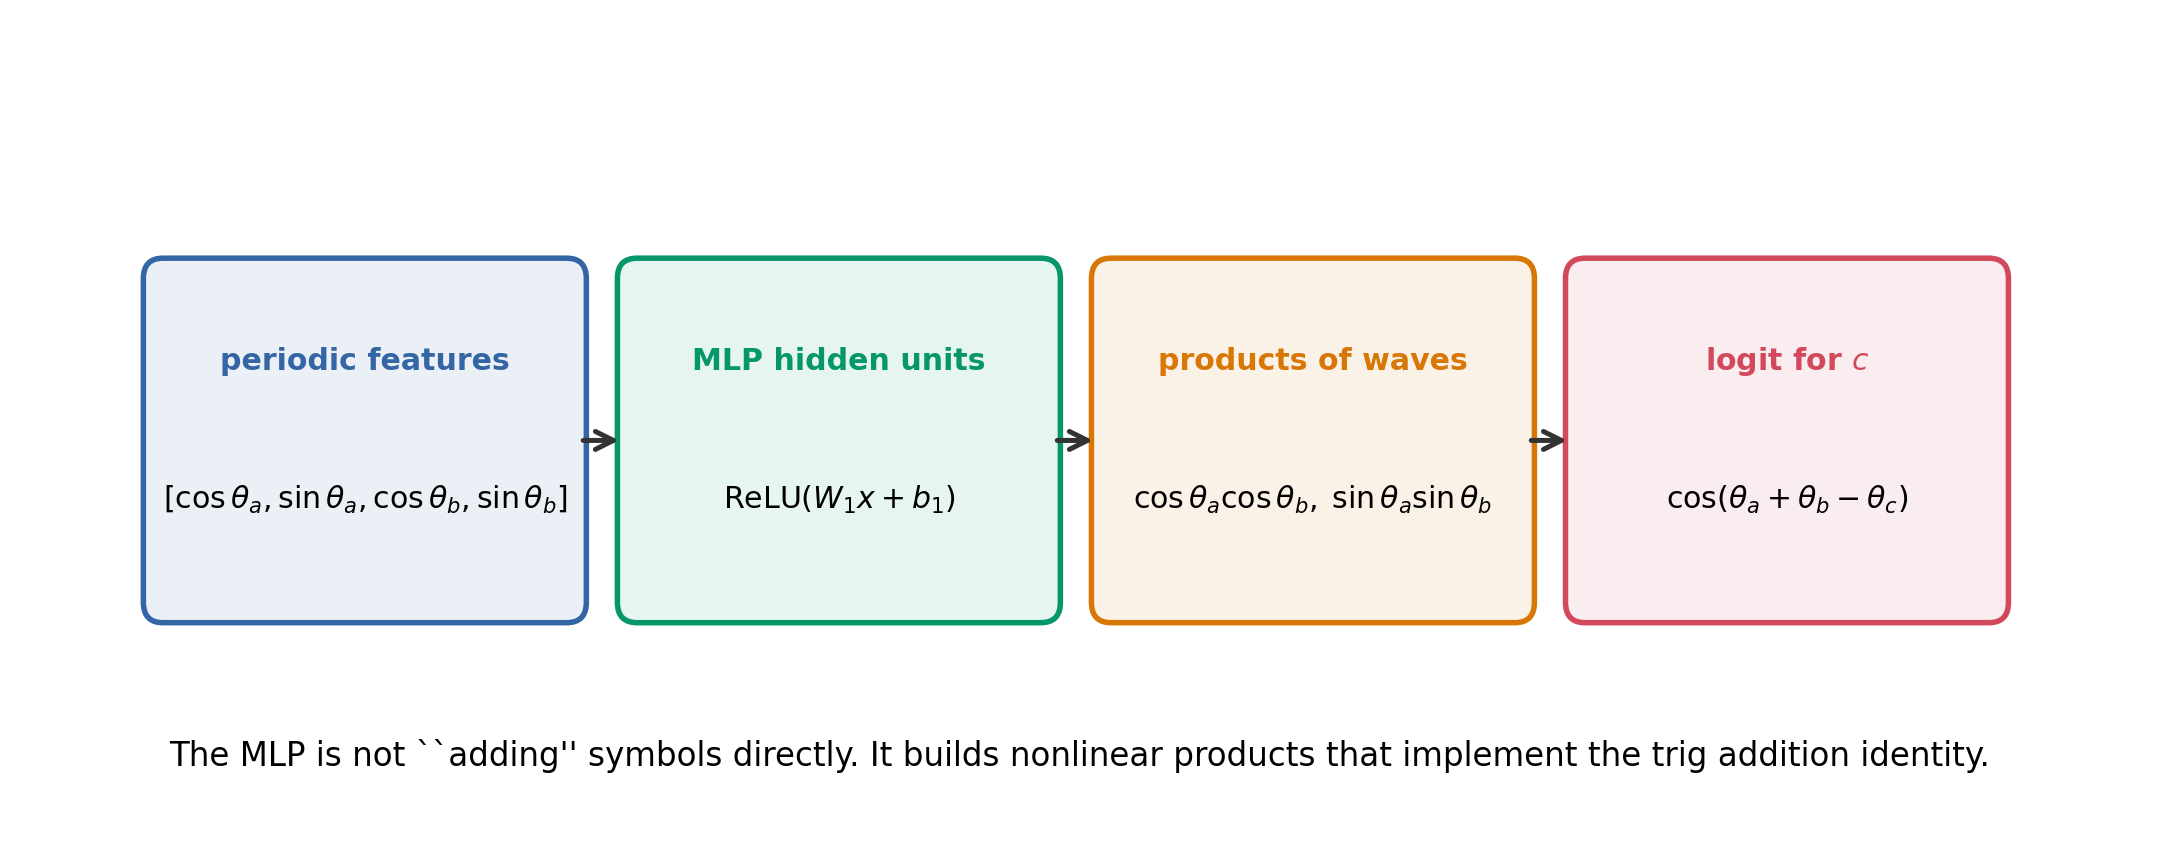
\includegraphics[width=.96\textwidth,height=.67\textheight,keepaspectratio]{fig/mlp_trig_mechanics.png}
\end{center}
\vfill
\small The diagram is a functional description. A ReLU MLP approximates these nonlinear combinations through many piecewise-linear hidden units; it is not a literal multiplication gate.
\end{frame}

\begin{frame}
\frametitle{Step 5: an unembedding turns the final vector into logits}
\begin{center}
\[
\mathrm{logits}=x_{=}^{(\mathrm{final})}W_U+b_U
\qquad\Longrightarrow\qquad
\Pr(c\mid a,b)=\mathrm{softmax}(\mathrm{logits})_c
\]
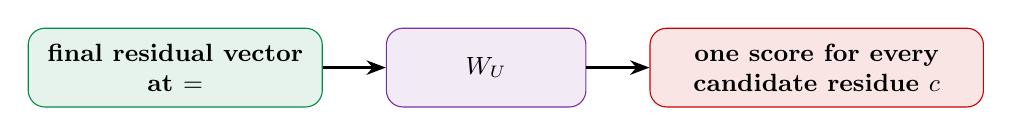
\begin{tikzpicture}[node distance=.8cm and .8cm]
\node[draw=paramgreen,fill=paramgreen!10,rounded corners=6pt,text width=3.5cm,minimum height=1.0cm,align=center,font=\small\bfseries] (res) {final residual vector\\at $=$};
\node[draw=violet1,fill=violet1!10,rounded corners=6pt,text width=2.3cm,minimum height=1.0cm,align=center,font=\small\bfseries,right=of res] (un) {$W_U$};
\node[draw=sampred,fill=sampred!10,rounded corners=6pt,text width=4.0cm,minimum height=1.0cm,align=center,font=\small\bfseries,right=of un] (logits) {one score for every\\candidate residue $c$};
\draw[-{Stealth[length=7pt]},thick] (res)--(un);
\draw[-{Stealth[length=7pt]},thick] (un)--(logits);
\end{tikzpicture}
\end{center}
\vfill
\small For $2+3$, interpretability can project an intermediate update through $W_U$ and ask: does it increase the logit for $5$?
\end{frame}

{
\usebackgroundtemplate{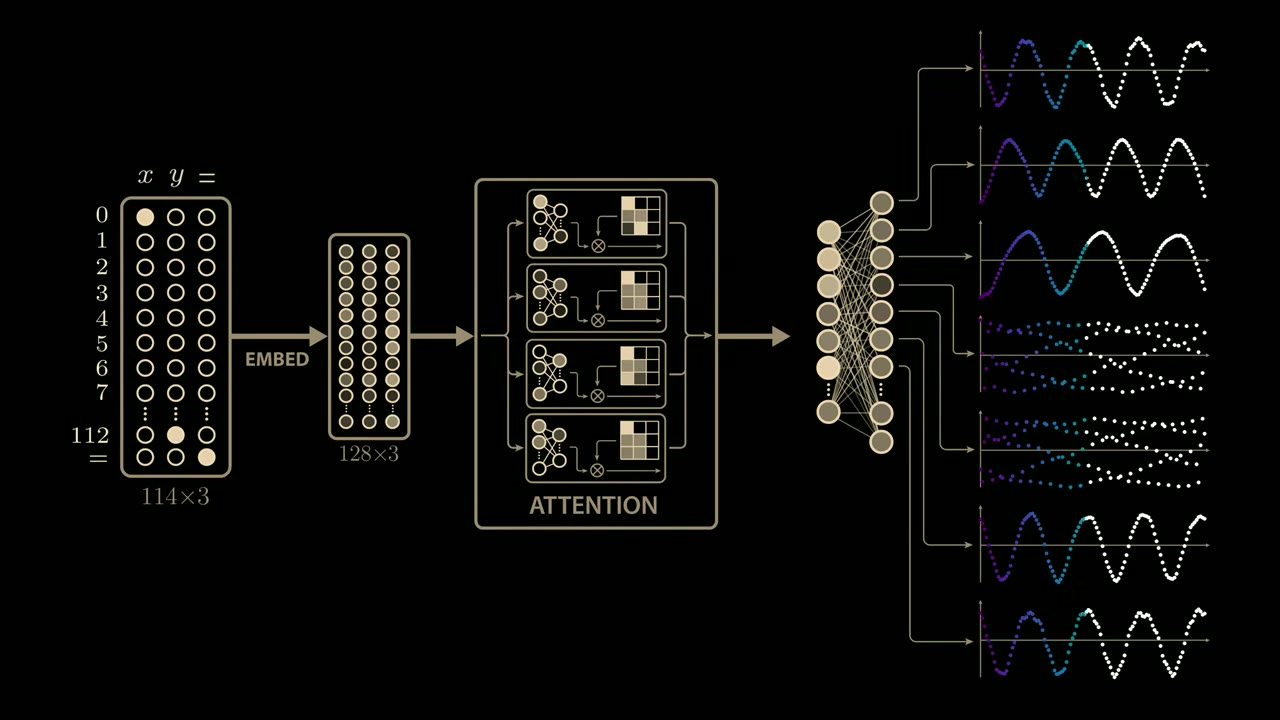
\includegraphics[width=\paperwidth,height=\paperheight]{../frames/f03_00-12-10.jpg}}
\begin{frame}[plain]
\source{Welch Labs, transformer and periodic activations, 12:10}
\end{frame}
}

% ----------------------------------------------------------------
\section{The identified circuit}
\transition{The identified modular-addition circuit}{We now leave generic transformer mechanics and ask what this trained model actually uses to solve modular addition.}

\begin{frame}
\frametitle{Three useful phases of grokking}
\begin{center}
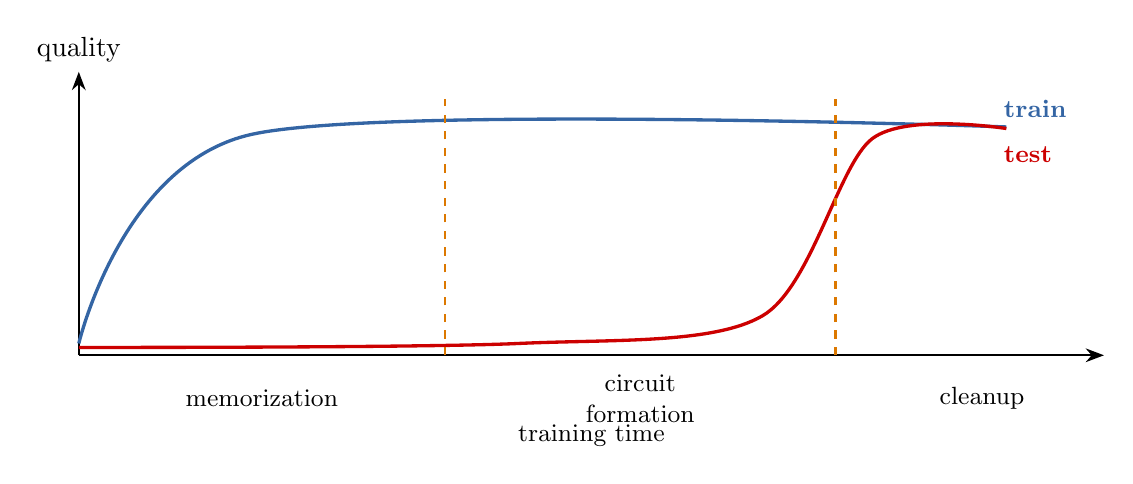
\begin{tikzpicture}[x=3.1cm,y=1cm]
\draw[-{Stealth},thick] (0,0)--(4.2,0);
\draw[-{Stealth},thick] (0,0)--(0,3.6) node[above]{quality};
\draw[popblue,very thick] plot[smooth] coordinates {(0,.15)(.7,2.8)(3.8,2.9)};
\draw[sampred,very thick] plot[smooth] coordinates {(0,.1)(1.8,.15)(2.8,.5)(3.25,2.75)(3.8,2.88)};
\draw[dashed,orange1,thick] (1.5,0)--(1.5,3.25);
\draw[dashed,orange1,thick] (3.1,0)--(3.1,3.25);
\node[align=center,font=\small] at (.75,-.55){memorization};
\node[align=center,font=\small] at (2.3,-.55){circuit\\formation};
\node[align=center,font=\small] at (3.7,-.55){cleanup};
\node[popblue,font=\small\bfseries,anchor=west] at (3.75,3.13){train};
\node[sampred,font=\small\bfseries,anchor=west] at (3.75,2.55){test};
\node[font=\small] at (2.1,-1.02){training time};
\end{tikzpicture}
\end{center}
\vspace{0.2cm}
\small Nanda et al. (2023): hidden progress can precede the visible accuracy transition.
\end{frame}

{
\usebackgroundtemplate{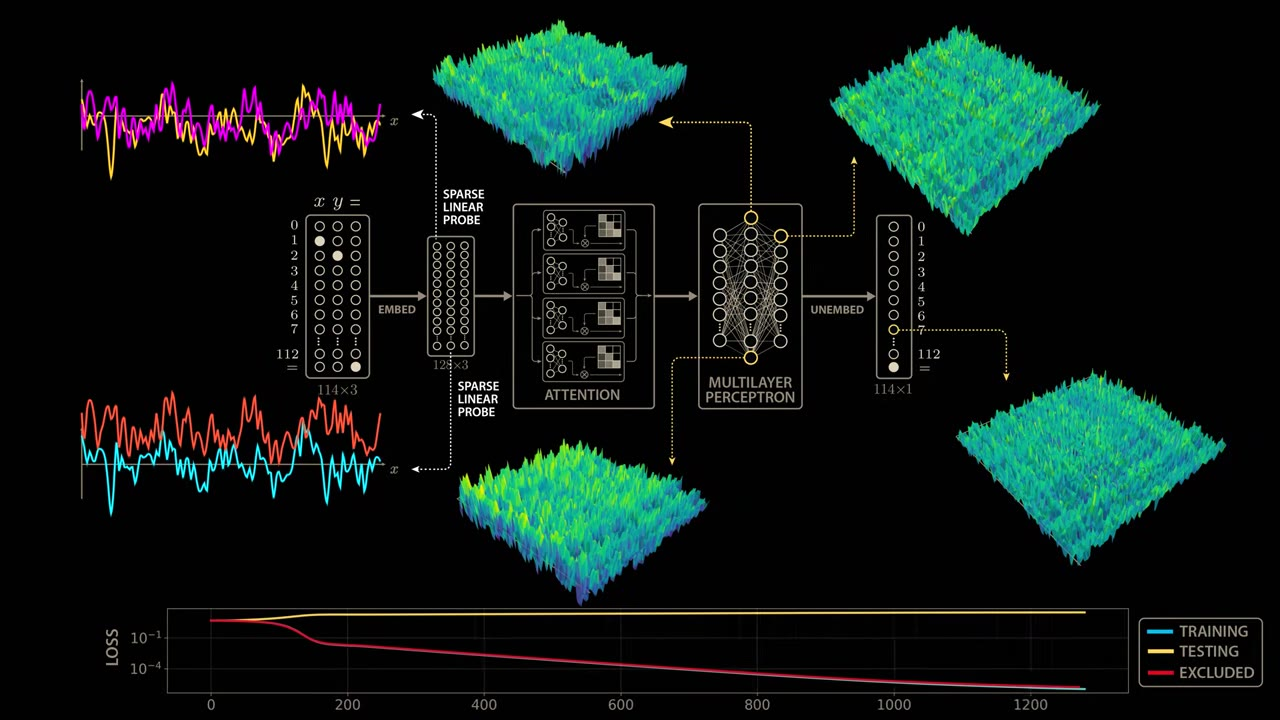
\includegraphics[width=\paperwidth,height=\paperheight]{../frames/f07_00-28-20.jpg}}
\begin{frame}[plain]
\source{Welch Labs, excluded-loss diagnostic, 28:20}
\end{frame}
}

\begin{frame}
\frametitle{What should we inspect inside the network?}
\begin{center}
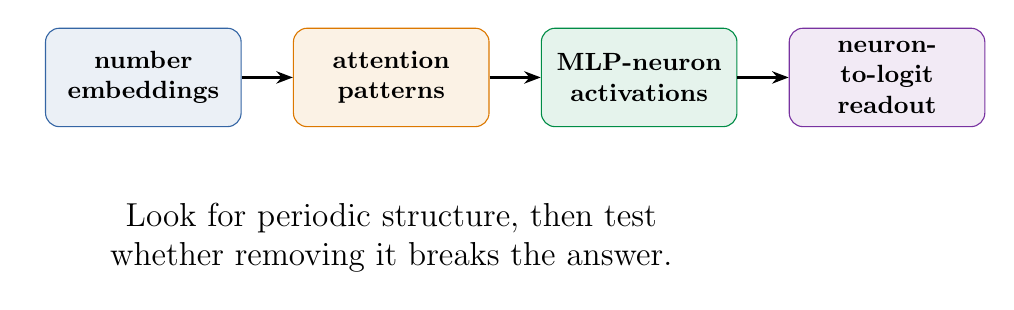
\begin{tikzpicture}[node distance=.75cm and .65cm]
\node[draw=popblue,fill=popblue!10,rounded corners=5pt,text width=2.25cm,minimum height=1.25cm,align=center,font=\small\bfseries] (e) {number embeddings};
\node[draw=orange1,fill=orange1!10,rounded corners=5pt,text width=2.25cm,minimum height=1.25cm,align=center,font=\small\bfseries,right=of e] (a) {attention patterns};
\node[draw=paramgreen,fill=paramgreen!10,rounded corners=5pt,text width=2.25cm,minimum height=1.25cm,align=center,font=\small\bfseries,right=of a] (m) {MLP-neuron activations};
\node[draw=violet1,fill=violet1!10,rounded corners=5pt,text width=2.25cm,minimum height=1.25cm,align=center,font=\small\bfseries,right=of m] (l) {neuron-to-logit readout};
\foreach \x/\y in {e/a,a/m,m/l} \draw[-{Stealth[length=6pt]},thick] (\x)--(\y);
\node[below=.85cm of a,align=center,text width=9cm,font=\large] {Look for periodic structure, then test whether removing it breaks the answer.};
\end{tikzpicture}
\end{center}
\end{frame}

{
\usebackgroundtemplate{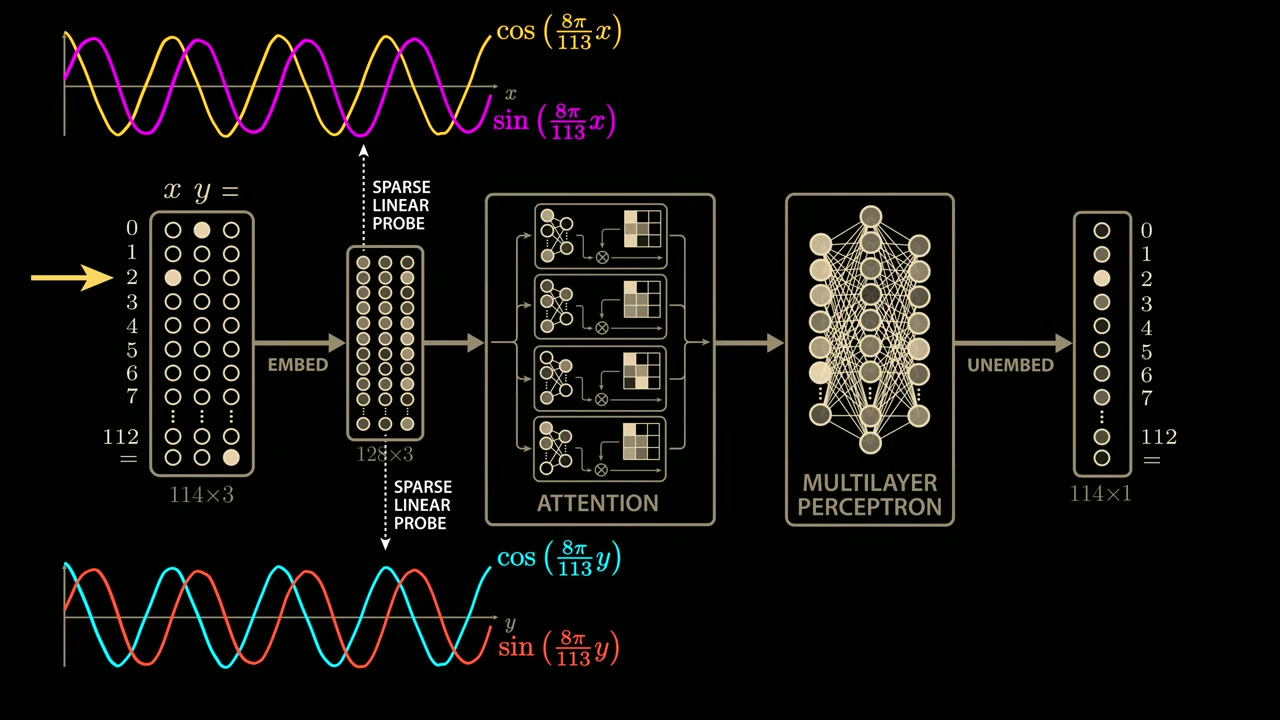
\includegraphics[width=\paperwidth,height=\paperheight]{../frames/f17_00-18-40.jpg}}
\begin{frame}[plain]
\source{Welch Labs, what to measure, 18:40}
\end{frame}
}

\begin{frame}
\frametitle{Checkpoint: what each part must contribute}
\begin{center}
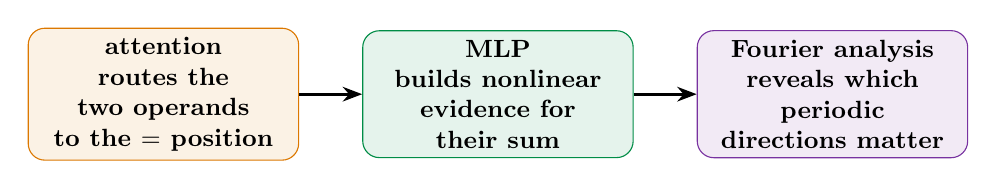
\begin{tikzpicture}[node distance=.65cm and .8cm]
\node[draw=orange1,fill=orange1!10,rounded corners=6pt,text width=3.2cm,minimum height=1.15cm,align=center,font=\small\bfseries] (attn) {attention\\routes the two operands\\to the $=$ position};
\node[draw=paramgreen,fill=paramgreen!10,rounded corners=6pt,text width=3.2cm,minimum height=1.15cm,align=center,font=\small\bfseries,right=of attn] (mlp) {MLP\\builds nonlinear\\evidence for their sum};
\node[draw=violet1,fill=violet1!10,rounded corners=6pt,text width=3.2cm,minimum height=1.15cm,align=center,font=\small\bfseries,right=of mlp] (fourier) {Fourier analysis\\reveals which periodic\\directions matter};
\draw[-{Stealth[length=7pt]},very thick] (attn)--(mlp);
\draw[-{Stealth[length=7pt]},very thick] (mlp)--(fourier);
\end{tikzpicture}
\end{center}
\vfill
\begin{center}\large For $2+3$, the circuit should create evidence specifically for $5$.\end{center}
\end{frame}

% ----------------------------------------------------------------
\section{Fourier transform}
\transition{Why Fourier transforms?}{They reveal circular patterns that are hard to see in raw coordinates.}

\begin{frame}
\frametitle{A Fourier transform asks: which simple waves make up this signal?}
\begin{center}
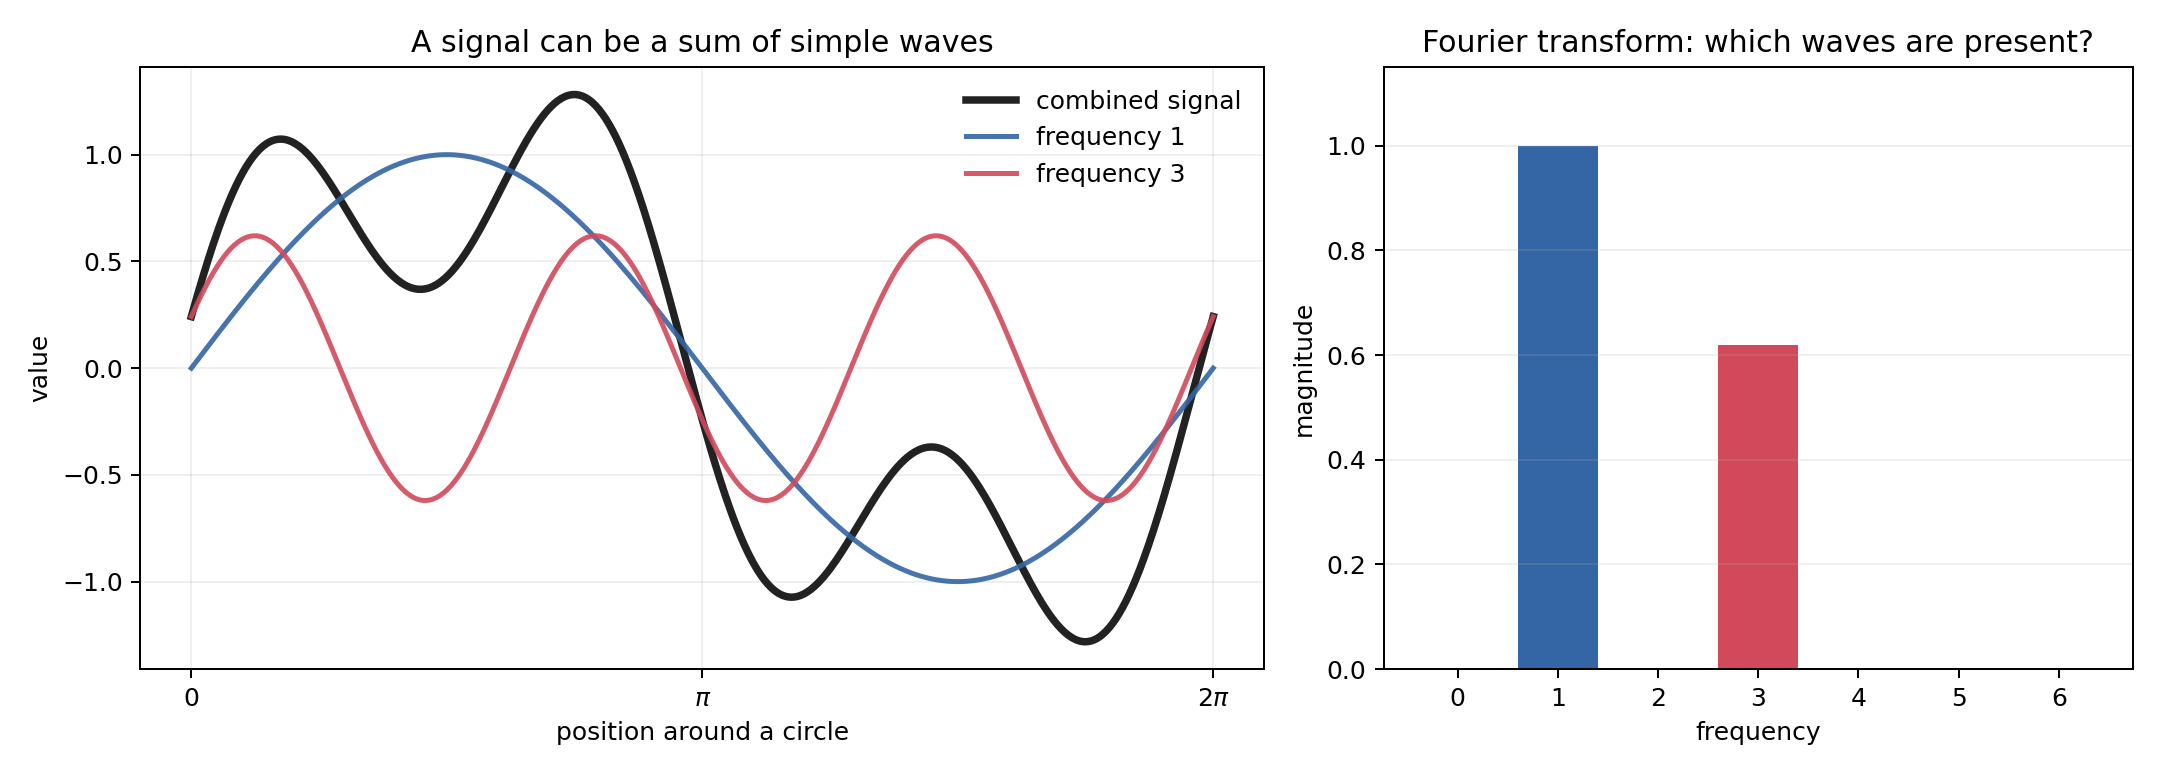
\includegraphics[width=.95\textwidth,height=.68\textheight,keepaspectratio]{fig/fourier_intro.png}
\end{center}
\vfill
\small Instead of describing a signal point-by-point, describe how strongly each frequency is present.
\end{frame}

\begin{frame}
\frametitle{A concrete example: a two-wave signal}
\begin{columns}[c]
\column{0.54\textwidth}
\[
f(x)=\sin x+0.62\sin(3x+0.4)
\]
\begin{itemize}\setlength\itemsep{0.48em}
\item The raw curve looks irregular because two motions are superposed.
\item The Fourier view separates it into frequency $1$ and frequency $3$.
\item The height and phase of each component summarize the whole signal.
\end{itemize}
\column{0.46\textwidth}
\begin{center}
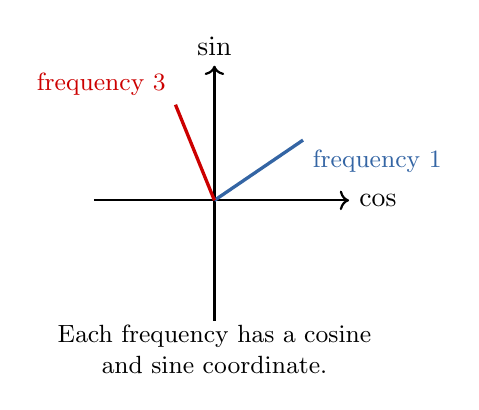
\begin{tikzpicture}[scale=.9]
\draw[->,thick] (-1.7,0)--(1.9,0) node[right] {$\cos$};
\draw[->,thick] (0,-1.7)--(0,1.9) node[above] {$\sin$};
\draw[popblue,very thick] (0,0)--(1.25,.85);
\draw[sampred,very thick] (0,0)--(-.55,1.35);
\node[popblue,below right,font=\small] at (1.25,.85) {frequency 1};
\node[sampred,above left,font=\small] at (-.55,1.35) {frequency 3};
\node[font=\small,align=center] at (0,-2.1) {Each frequency has a cosine\\and sine coordinate.};
\end{tikzpicture}
\end{center}
\end{columns}
\end{frame}

\begin{frame}
\frametitle{Bridge: the DFT receives one value for every residue token}
\begin{center}
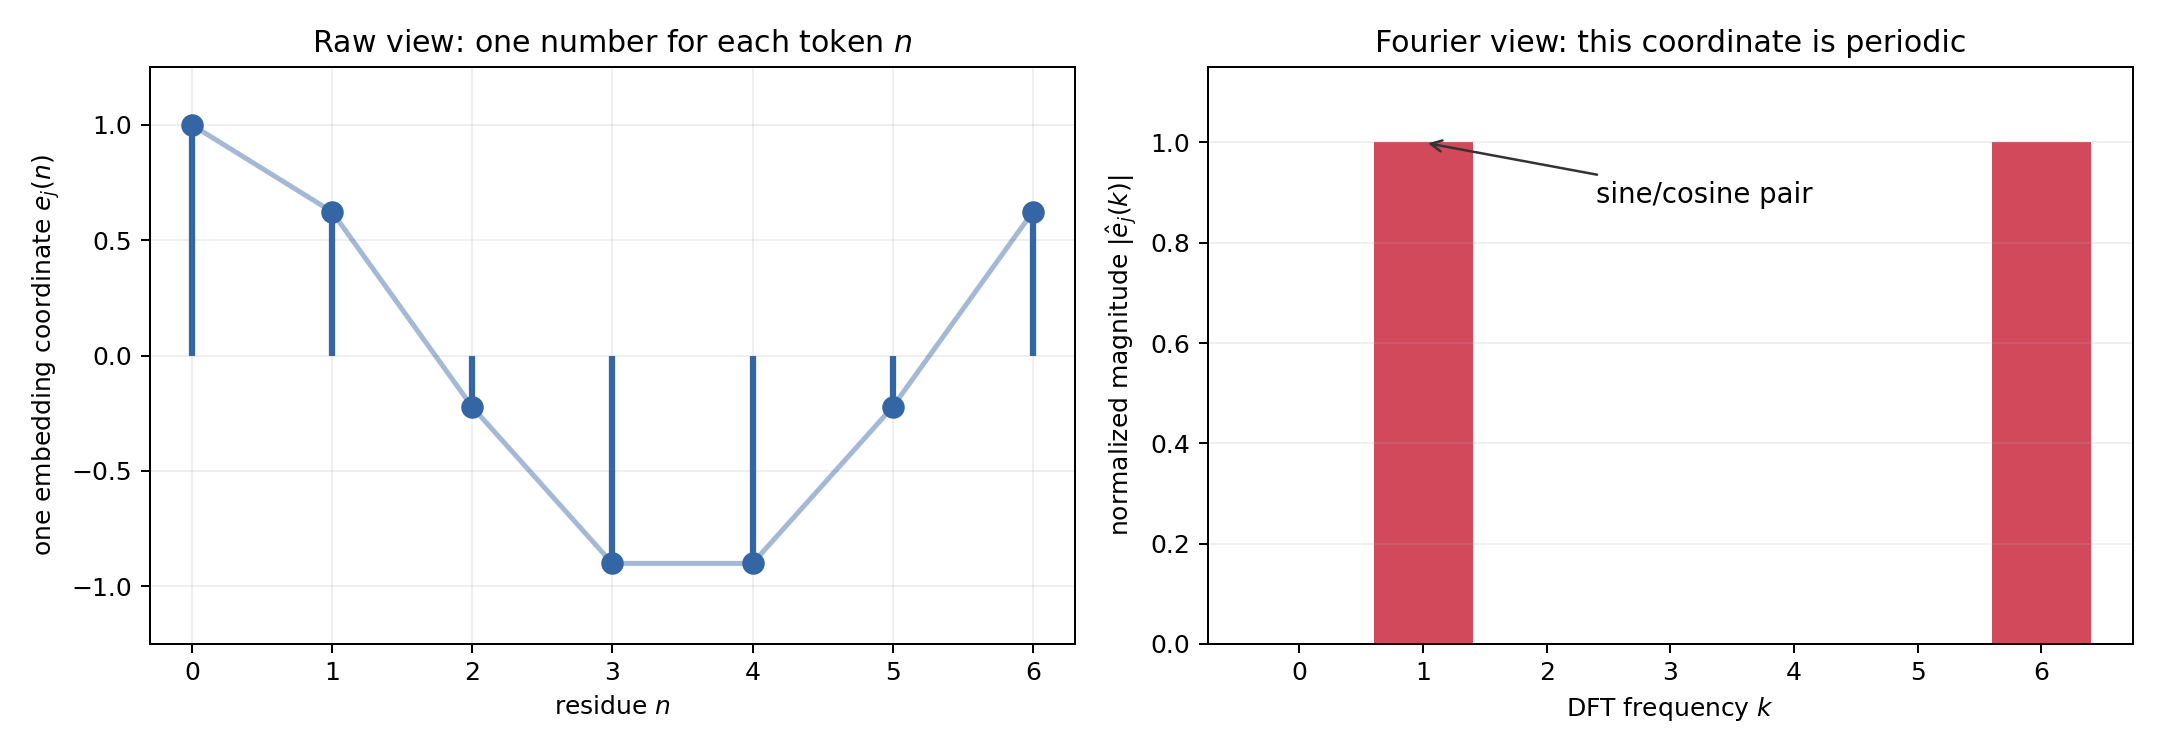
\includegraphics[width=.96\textwidth,height=.68\textheight,keepaspectratio]{fig/fourier_token_bridge.png}
\end{center}
\vfill
\small For an embedding coordinate $e_j$, treat $e_j(0),\ldots,e_j(P-1)$ as a discrete signal over token IDs. The DFT asks whether it traces a simple cycle around the modular circle.
\end{frame}

\begin{frame}
\frametitle{For modular arithmetic, use the discrete Fourier transform}
\begin{center}
\[
\widehat{x}_k=\sum_{n=0}^{P-1}x_n\,e^{-2\pi i kn/P},
\qquad k=0,\ldots,P-1
\]
\end{center}
\begin{columns}[T]
\column{0.5\textwidth}
\begin{block}{Input}
Take a quantity defined for each residue $n\in\{0,\ldots,P-1\}$: an embedding coordinate, neuron activation, or output logit.
\end{block}
\column{0.5\textwidth}
\begin{block}{Output}
For each frequency $k$, $\widehat{x}_k$ records the strength and phase of a wave as we walk around the modular circle.
\end{block}
\end{columns}
\vfill
\small In a real-valued model, the useful basis appears as sine/cosine pairs rather than complex numbers.
\end{frame}

\begin{frame}
\frametitle{Why a sine/cosine pair is a circular coordinate system}
\begin{columns}[c]
\column{0.48\textwidth}
\[
n\longmapsto
\left(
\cos\frac{2\pi kn}{P},
\sin\frac{2\pi kn}{P}
\right)
\]
\begin{itemize}\setlength\itemsep{0.5em}
\item $k$ says how many turns the wave completes around the residue circle.
\item The pair retains phase: where the wave is on the circle.
\item Addition of residues becomes addition of angles.
\end{itemize}
\column{0.52\textwidth}
\begin{center}
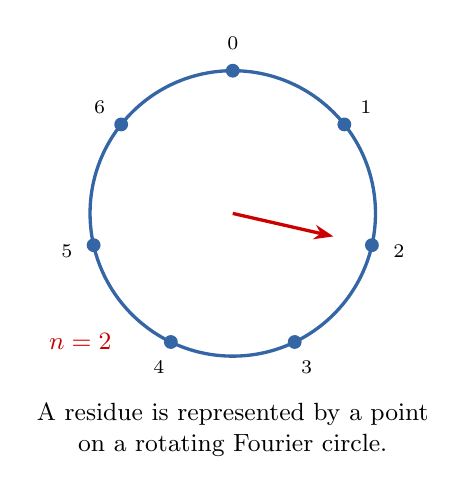
\begin{tikzpicture}[scale=1.25]
\draw[very thick,popblue] (0,0) circle (1.45);
\foreach \n in {0,...,6}{\pgfmathsetmacro{\ang}{90-360*\n/7}\fill[popblue] ({1.45*cos(\ang)},{1.45*sin(\ang)}) circle (2pt);\node[font=\scriptsize] at ({1.73*cos(\ang)},{1.73*sin(\ang)}) {\n};}
\draw[-{Stealth[length=7pt]},very thick,sampred] (0,0)--({1.05*cos(90-360*2/7)},{1.05*sin(90-360*2/7)});
\node[sampred,font=\small\bfseries] at (-1.55,-1.3) {$n=2$};
\node[font=\small,align=center] at (0,-2.2) {A residue is represented by a point\\on a rotating Fourier circle.};
\end{tikzpicture}
\end{center}
\end{columns}
\end{frame}

{
\usebackgroundtemplate{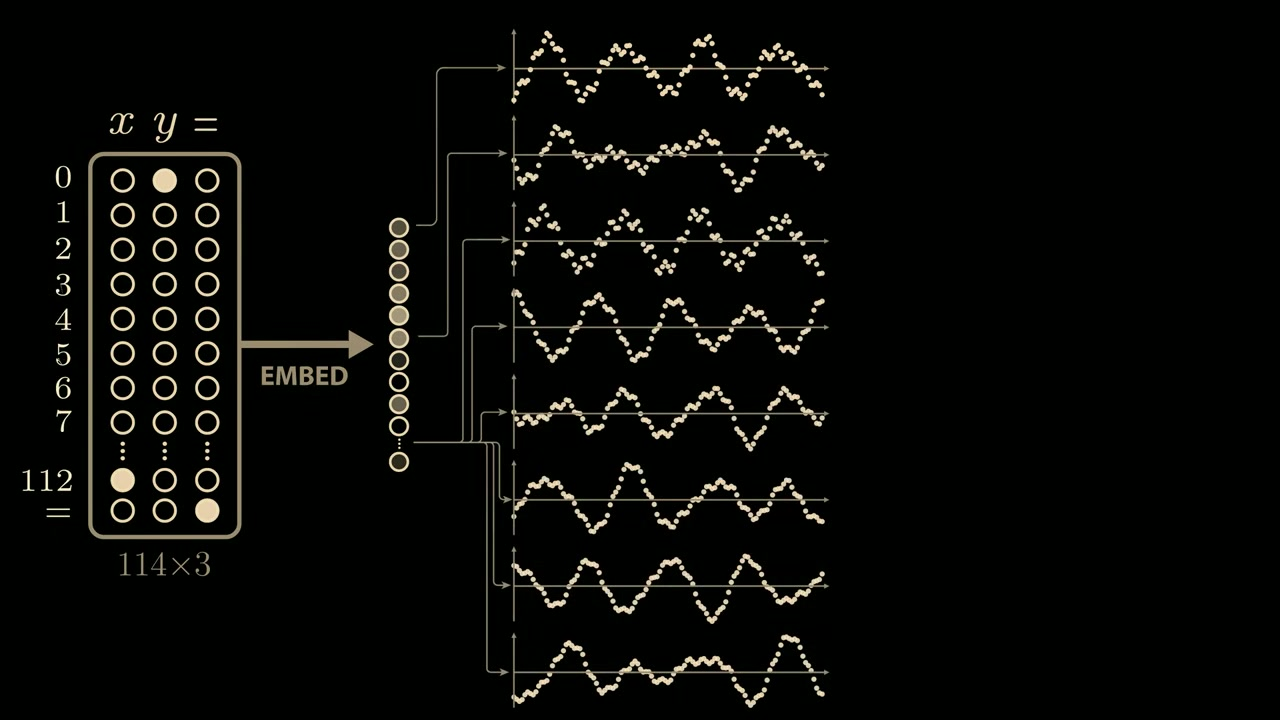
\includegraphics[width=\paperwidth,height=\paperheight]{../frames/f16_00-15-40.jpg}}
\begin{frame}[plain]
\source{Welch Labs, periodic representations, 15:40}
\end{frame}
}

\begin{frame}
\frametitle{The mechanistic finding: a small set of Fourier modes dominates}
\begin{columns}[c]
\column{0.51\textwidth}
\begin{itemize}\setlength\itemsep{0.5em}
\item Fourier analysis reveals periodic directions in embeddings, MLP activations, and logits.
\item Only a few frequencies carry most of the modular-addition computation.
\item This turns an enormous parameter set into a compact candidate circuit.
\end{itemize}
\column{0.49\textwidth}
\begin{center}
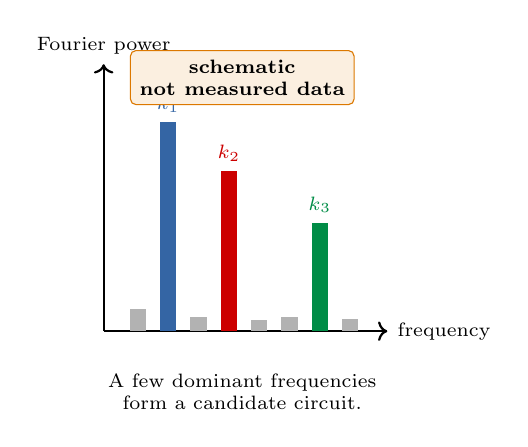
\begin{tikzpicture}[x=.55cm,y=1.13cm]
\draw[->,thick] (0,0)--(6.55,0) node[right,font=\scriptsize]{frequency};
\draw[->,thick] (0,0)--(0,3.0) node[above,font=\scriptsize]{Fourier power};
\foreach \x/\h/\c in {.6/.25/black!30,1.3/2.35/popblue,2.0/.16/black!30,2.7/1.8/sampred,3.4/.12/black!30,4.1/.16/black!30,4.8/1.22/paramgreen,5.5/.14/black!30}{\fill[\c] (\x,0) rectangle +(.38,\h);}
\node[popblue,font=\scriptsize,above] at (1.49,2.35) {$k_1$};
\node[sampred,font=\scriptsize,above] at (2.89,1.8) {$k_2$};
\node[paramgreen,font=\scriptsize,above] at (4.99,1.22) {$k_3$};
\node[draw=orange1,fill=orange1!12,rounded corners=2pt,font=\scriptsize\bfseries,align=center] at (3.2,2.85) {schematic\\not measured data};
\node[font=\scriptsize,align=center] at (3.2,-.68) {A few dominant frequencies\\form a candidate circuit.};
\end{tikzpicture}
\end{center}
\end{columns}
\vfill
\small Nanda et al. (2023) use Fourier structure together with causal interventions, not Fourier plots alone.
\end{frame}

{
\usebackgroundtemplate{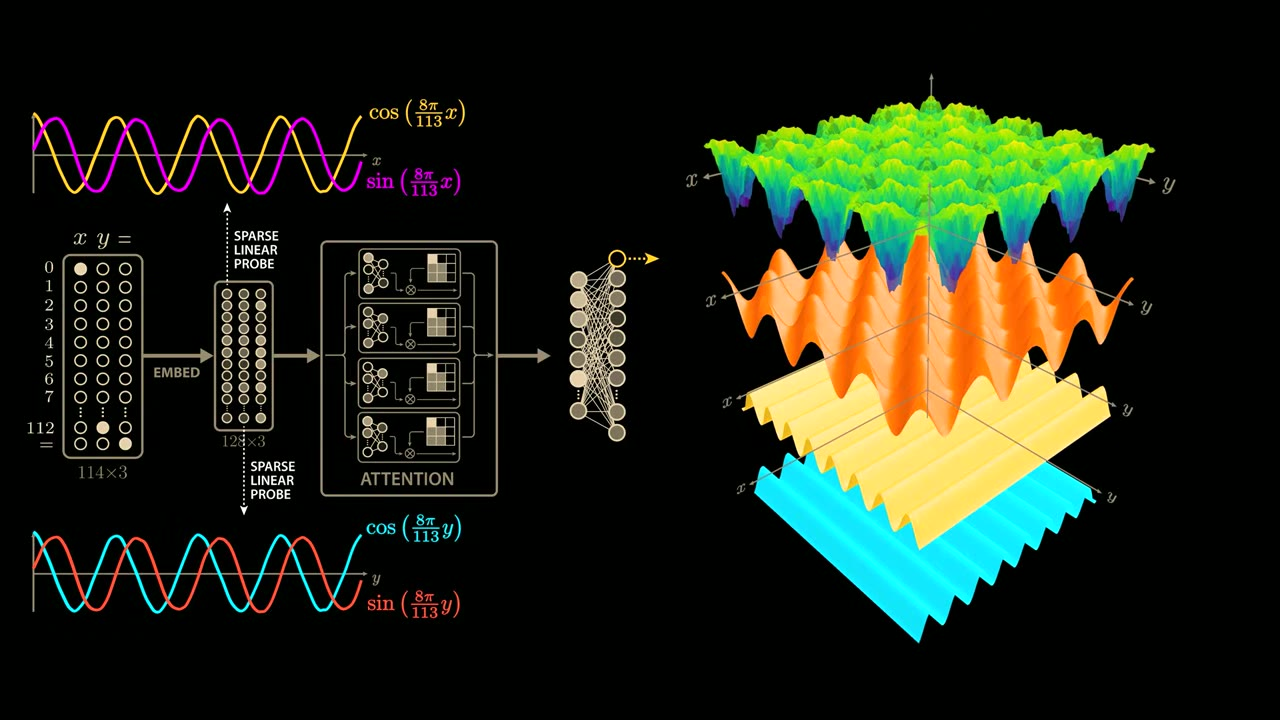
\includegraphics[width=\paperwidth,height=\paperheight]{../frames/f05_00-20-30.jpg}}
\begin{frame}[plain]
\source{Welch Labs, probes and frequency surfaces, 20:30}
\end{frame}
}

{
\usebackgroundtemplate{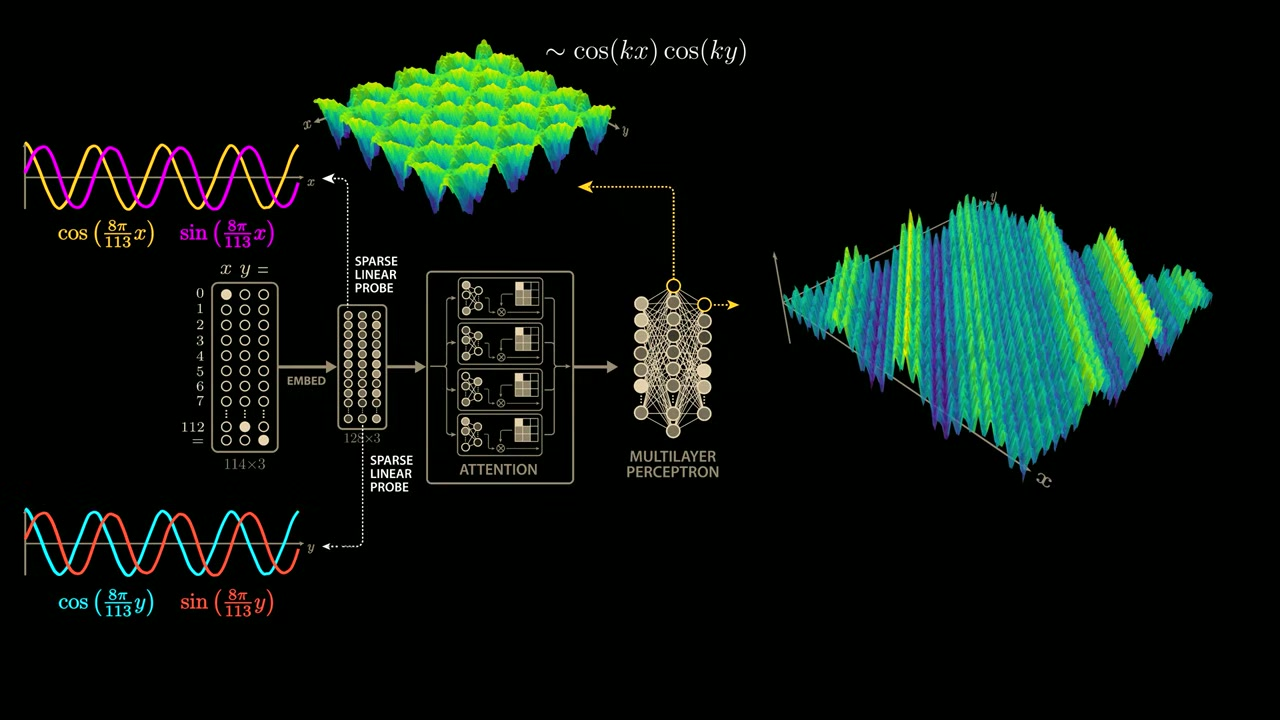
\includegraphics[width=\paperwidth,height=\paperheight]{../frames/f18_00-21-40.jpg}}
\begin{frame}[plain]
\source{Welch Labs, Fourier components, 21:40}
\end{frame}
}

% ----------------------------------------------------------------
\section{The modular-addition mechanism}
\transition{A clock turns addition into rotation}{The Fourier basis makes the arithmetic rule geometrically simple.}

\begin{frame}
\frametitle{Numbers modulo $P$ live naturally on a clock}
\begin{columns}[c]
\column{0.52\textwidth}
\begin{center}
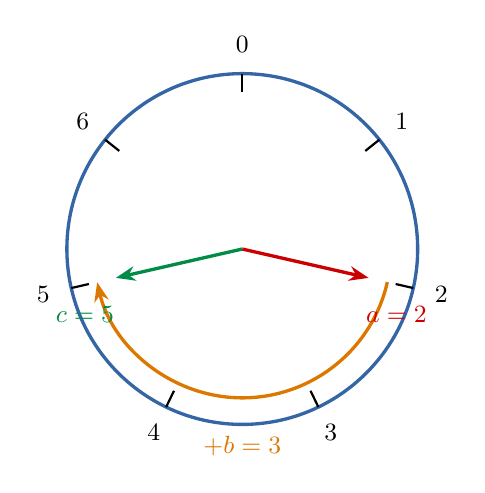
\begin{tikzpicture}[scale=1.35]
\draw[very thick,popblue] (0,0) circle (1.65);
\foreach \n in {0,...,6}{\pgfmathsetmacro{\ang}{90-360*\n/7}\draw[thick] ({1.48*cos(\ang)},{1.48*sin(\ang)})--({1.65*cos(\ang)},{1.65*sin(\ang)});\node[font=\small] at ({1.92*cos(\ang)},{1.92*sin(\ang)}) {\n};}
\draw[-{Stealth[length=7pt]},very thick,sampred] (0,0)--({1.22*cos(90-360*2/7)},{1.22*sin(90-360*2/7)});
\draw[-{Stealth[length=7pt]},very thick,orange1] ({1.40*cos(90-360*2/7)},{1.40*sin(90-360*2/7)}) arc[start angle={90-360*2/7},end angle={90-360*5/7},radius=1.40];
\draw[-{Stealth[length=7pt]},very thick,paramgreen] (0,0)--({1.22*cos(90-360*5/7)},{1.22*sin(90-360*5/7)});
\node[sampred,font=\small\bfseries] at (1.45,-.62) {$a=2$};
\node[orange1,font=\small\bfseries] at (0,-1.85) {$+b=3$};
\node[paramgreen,font=\small\bfseries] at (-1.48,-.62) {$c=5$};
\end{tikzpicture}
\end{center}
\column{0.48\textwidth}
\begin{block}{Rotation view}
Represent $n$ by the angle $2\pi n/P$.
\end{block}
\[
\theta_{2+3}=\theta_2+\theta_3 \pmod{2\pi}
\]
Adding residues becomes adding angles around a circle.
\end{columns}
\end{frame}

{
\usebackgroundtemplate{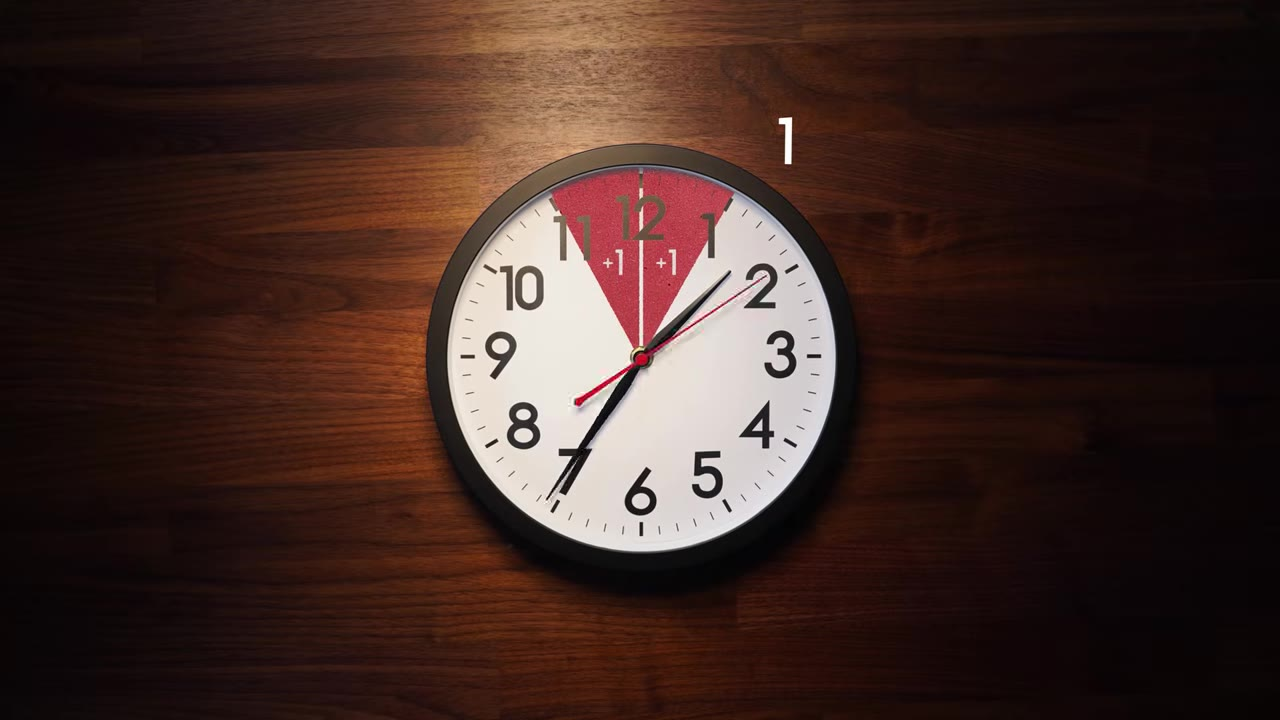
\includegraphics[width=\paperwidth,height=\paperheight]{../frames/f04_00-17-30.jpg}}
\begin{frame}[plain]
\source{Welch Labs, clock analogy, 17:30}
\end{frame}
}

\begin{frame}
\frametitle{The trigonometric identity that composes rotations}
\begin{center}\Large\[
\begin{aligned}
\cos(x+y) &= \cos x\cos y - \sin x\sin y\\[0.45cm]
\sin(x+y) &= \sin x\cos y + \cos x\sin y
\end{aligned}\]
\end{center}
\begin{columns}[T]
\column{0.5\textwidth}
\begin{block}{Input features}
Encode $a$ and $b$ as $(\cos\theta_a,\sin\theta_a)$ and $(\cos\theta_b,\sin\theta_b)$.
\end{block}
\column{0.5\textwidth}
\begin{block}{Answer score}
For candidate $c$, a natural score is $\cos(\theta_a+\theta_b-\theta_c)$, highest when $c=a+b$.
\end{block}
\end{columns}
\end{frame}

\begin{frame}
\frametitle{Worked score: why $c=5$ wins for $2+3$ modulo $7$}
\begin{columns}[T]
\column{0.48\textwidth}
\[
\theta_n=\frac{2\pi n}{7}
\]
\[
\theta_2=\frac{4\pi}{7},\qquad
\theta_3=\frac{6\pi}{7},\qquad
\theta_5=\frac{10\pi}{7}
\]
\column{0.52\textwidth}
\[
\mathrm{score}(c)=\cos(\theta_2+\theta_3-\theta_c)
\]
\[
\mathrm{score}(5)=\cos(0)=1
\]
\[
\mathrm{score}(4)=\cos\left(\frac{2\pi}{7}\right)<1
\]
\end{columns}
\vfill
\small Attention brings periodic features for $2$ and $3$ together. The MLP approximates the products in the trig identity, and the unembedding compares the resulting phase with every candidate $c$.
\end{frame}

\begin{frame}
\frametitle{A Fourier-style circuit for modular addition}
\begin{center}
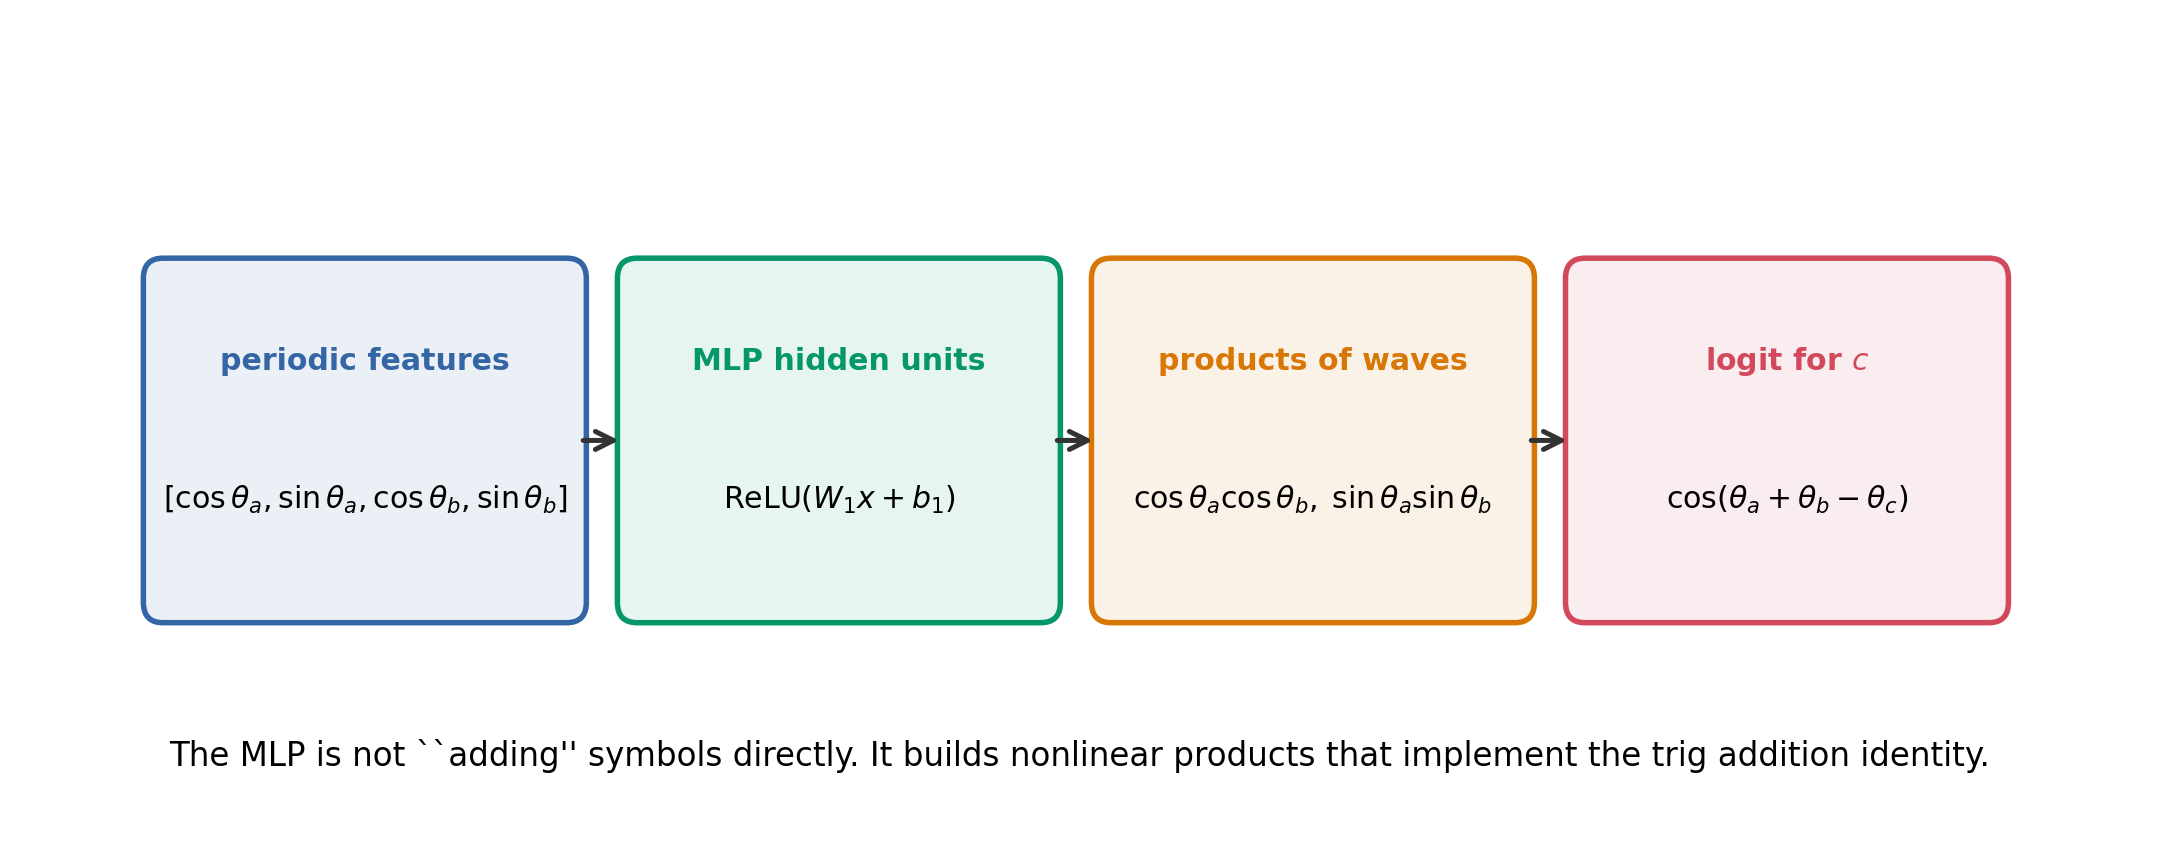
\includegraphics[width=.96\textwidth,height=.67\textheight,keepaspectratio]{fig/mlp_trig_mechanics.png}
\end{center}
\vfill
\small For every useful frequency, the network can vote for the candidate whose phase matches the summed input phase. Several frequencies make that vote more specific.
\end{frame}

{
\usebackgroundtemplate{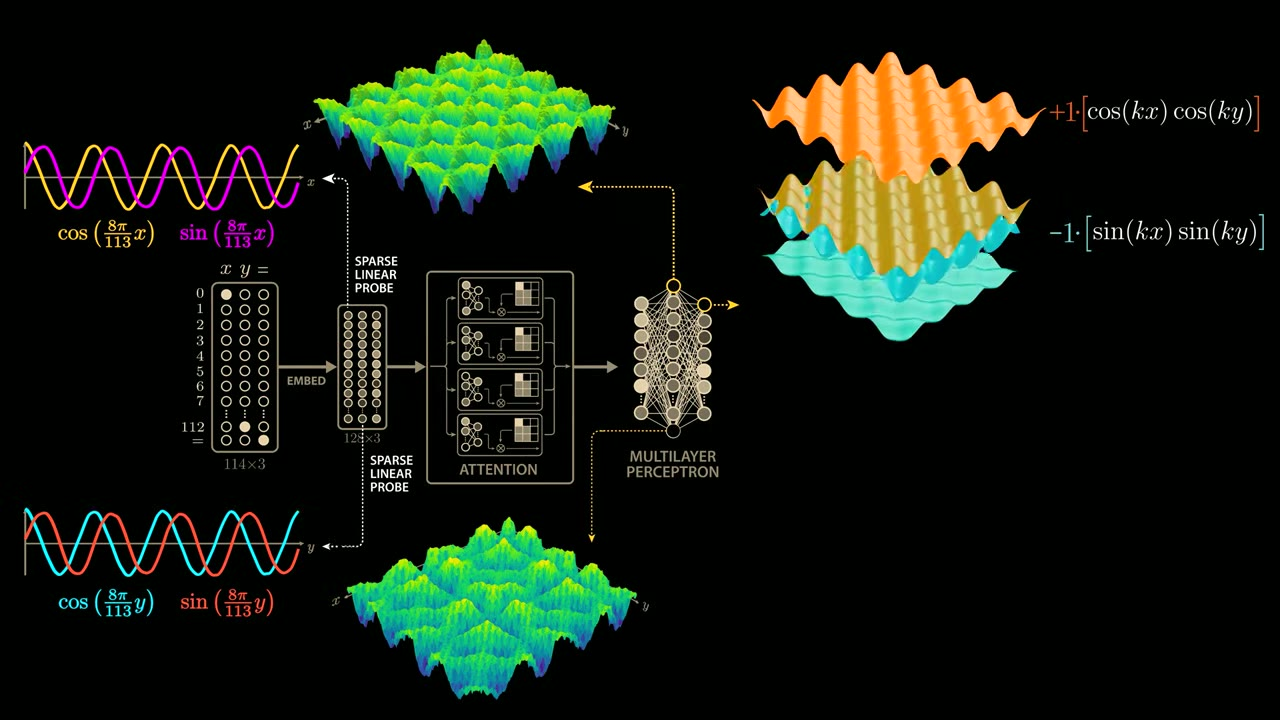
\includegraphics[width=\paperwidth,height=\paperheight]{../frames/f06_00-24-25.jpg}}
\begin{frame}[plain]
\source{Welch Labs, trigonometric mechanism, 24:25}
\end{frame}
}

{
\usebackgroundtemplate{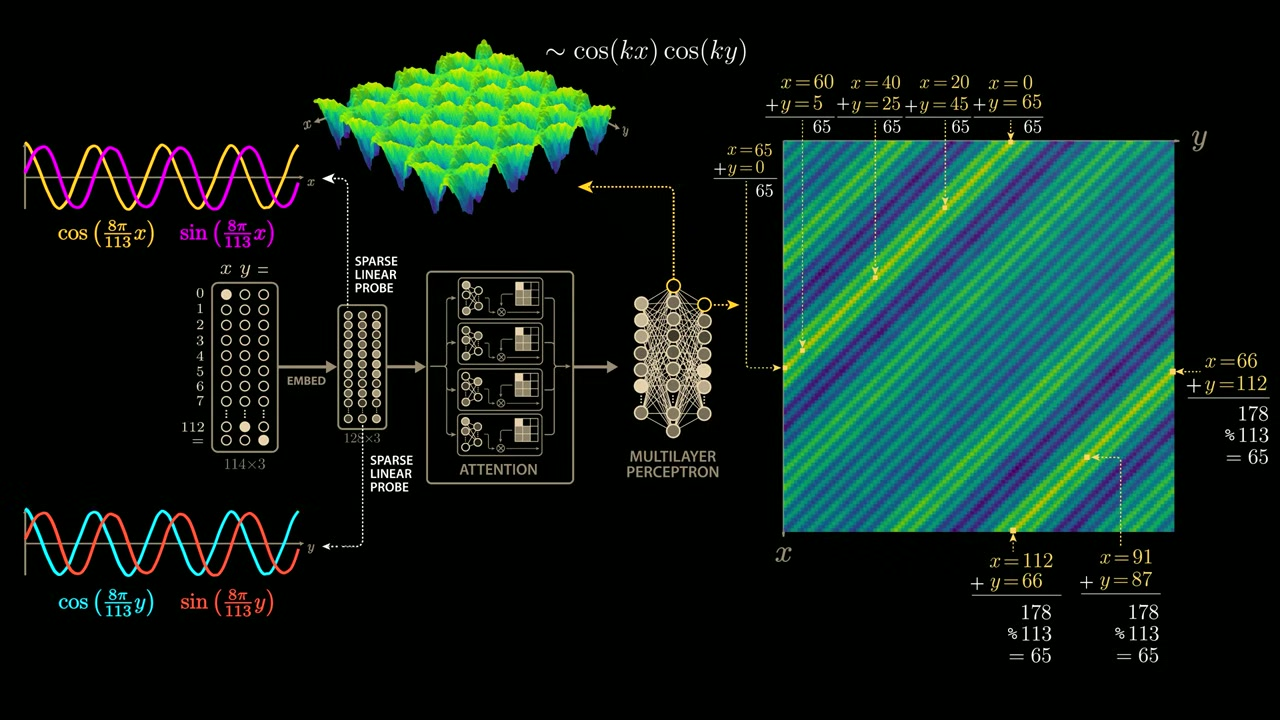
\includegraphics[width=\paperwidth,height=\paperheight]{../frames/f19_00-23-10.jpg}}
\begin{frame}[plain]
\source{Welch Labs, circuit-level interpretation, 23:10}
\end{frame}
}

\begin{frame}
\frametitle{A causal explanation needs interventions}
\begin{columns}[c]
\column{0.48\textwidth}
\begin{itemize}\setlength\itemsep{0.65em}
\item Fourier-transform embeddings and logits.
\item Identify a few key frequencies.
\item Keep only those frequencies: performance remains.
\item Remove them: performance collapses.
\end{itemize}
\column{0.52\textwidth}
\begin{center}
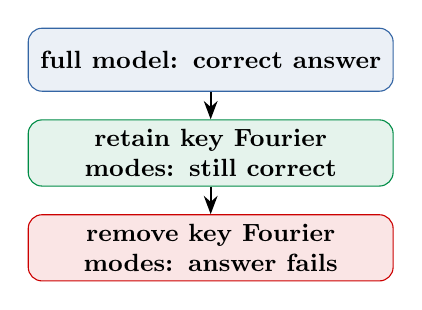
\begin{tikzpicture}[node distance=.35cm]
\node[draw=popblue,fill=popblue!10,rounded corners=5pt,text width=4.4cm,minimum height=0.8cm,align=center,font=\small\bfseries] (full) {full model: correct answer};
\node[draw=paramgreen,fill=paramgreen!10,rounded corners=5pt,text width=4.4cm,minimum height=0.8cm,align=center,font=\small\bfseries,below=of full] (keep) {retain key Fourier modes: still correct};
\node[draw=sampred,fill=sampred!10,rounded corners=5pt,text width=4.4cm,minimum height=0.8cm,align=center,font=\small\bfseries,below=of keep] (drop) {remove key Fourier modes: answer fails};
\draw[-{Stealth},thick] (full)--(keep);\draw[-{Stealth},thick] (keep)--(drop);
\end{tikzpicture}
\end{center}
\end{columns}
\vfill\small Nanda et al. (2023): this is the evidence standard. A periodic-looking plot alone does not establish a mechanism.
\end{frame}

{
\usebackgroundtemplate{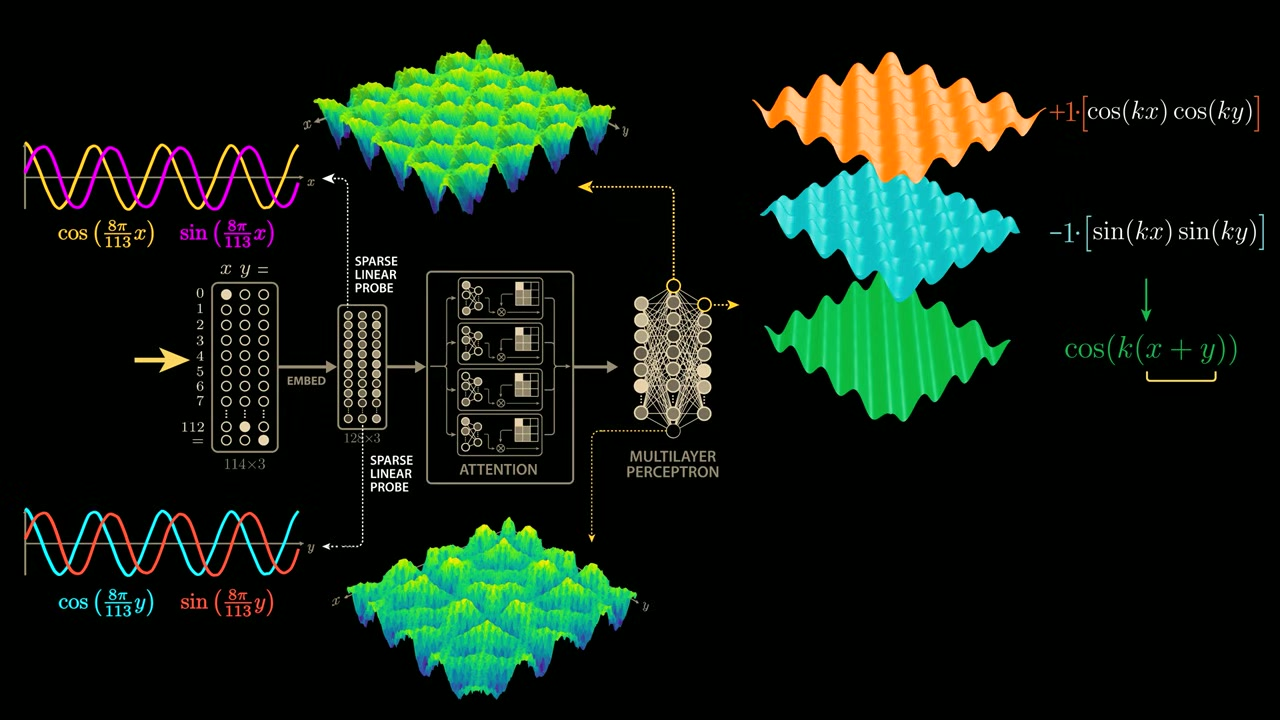
\includegraphics[width=\paperwidth,height=\paperheight]{../frames/f20_00-25-20.jpg}}
\begin{frame}[plain]
\source{Welch Labs, causal tests, 25:20}
\end{frame}
}

% ----------------------------------------------------------------
\section{From a toy model to Claude}
\transition{From a toy model to Claude}{Different task, different evidence: this is not a second grokking result. The interpretability questions transfer, but the mechanisms are less neatly localized.}

\begin{frame}
\frametitle{Claude Haiku: a line-break counting manifold}
\begin{columns}[T]
\column{0.52\textwidth}
\begin{itemize}\setlength\itemsep{0.5em}
\item Claude 3.5 Haiku adapts to different target line widths.
\item Internal representations track position within the line and the width target.
\item The relevant states form a geometric counting manifold, not one isolated newline neuron.
\end{itemize}
\column{0.48\textwidth}
\begin{center}
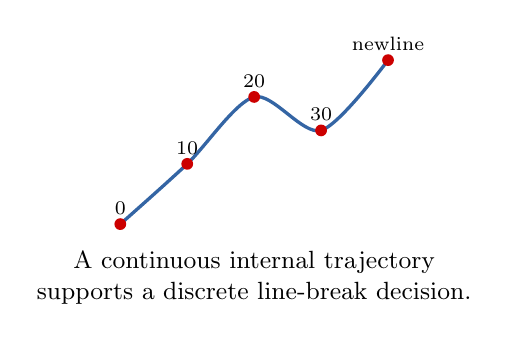
\begin{tikzpicture}[scale=.85]
\draw[popblue,very thick] plot[smooth] coordinates {(-2,-1.2)(-1,-.3)(0,.7)(1,.2)(2,1.25)};
\foreach \x/\y/\t in {-2/-1.2/0,-1/-.3/10,0/.7/20,1/.2/30,2/1.25/newline}{\fill[sampred] (\x,\y) circle (2.5pt);\node[font=\scriptsize,above] at (\x,\y) {\t};}
\node[align=center,font=\small] at (0,-2) {A continuous internal trajectory\\supports a discrete line-break decision.};
\end{tikzpicture}
\end{center}
\end{columns}
\vfill\small Gurnee et al. (2025), \textit{When Models Manipulate Manifolds}.
\end{frame}

{
\usebackgroundtemplate{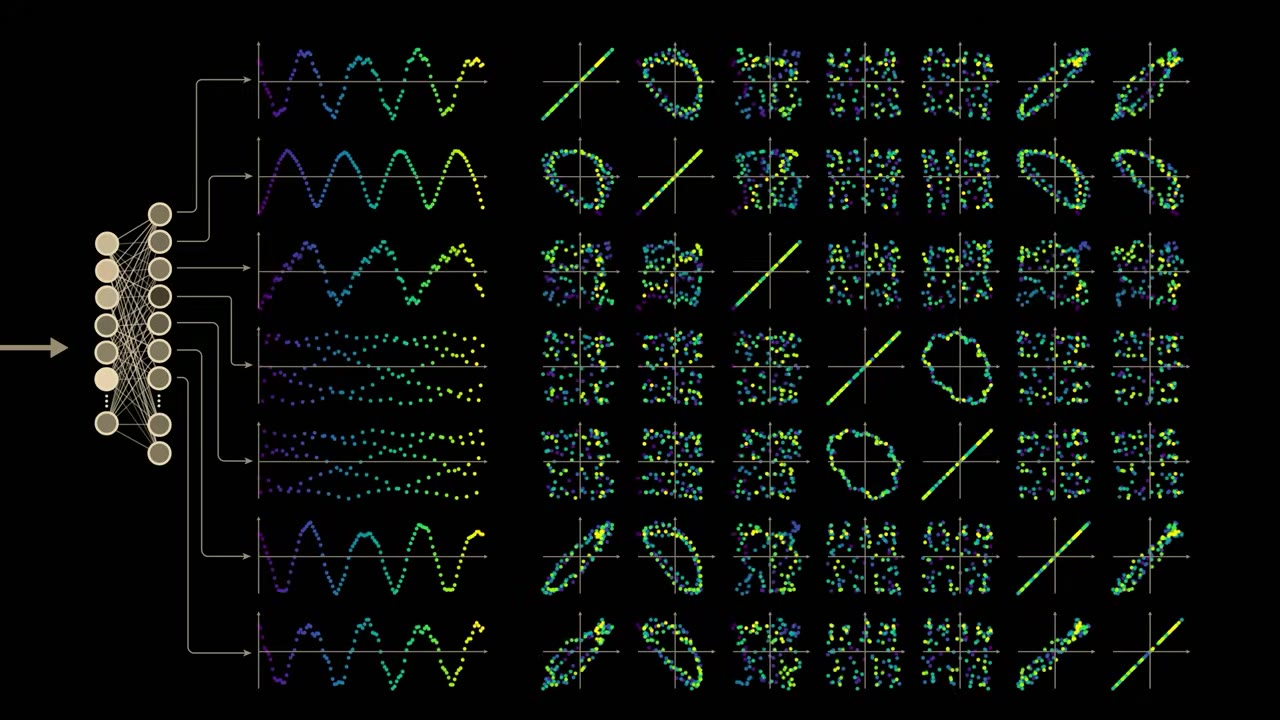
\includegraphics[width=\paperwidth,height=\paperheight]{../frames/f08_00-30-35.jpg}}
\begin{frame}[plain]
\source{Welch Labs, Claude Haiku comparison, 30:35}
\end{frame}
}

{
\usebackgroundtemplate{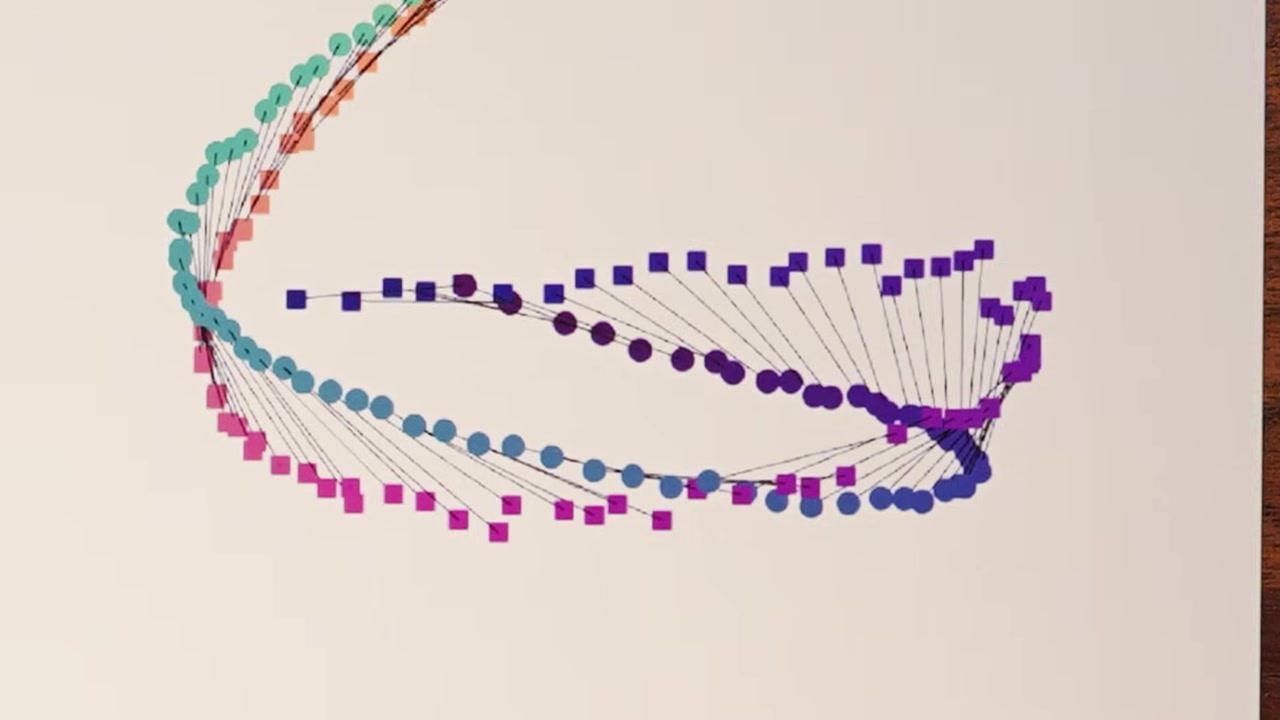
\includegraphics[width=\paperwidth,height=\paperheight]{../frames/f22_00-31-30.jpg}}
\begin{frame}[plain]
\source{Welch Labs, feature geometry, 31:30}
\end{frame}
}

\begin{frame}
\frametitle{Superposition: many feature directions, few dimensions}
\begin{columns}[c]
\column{0.48\textwidth}
\begin{center}
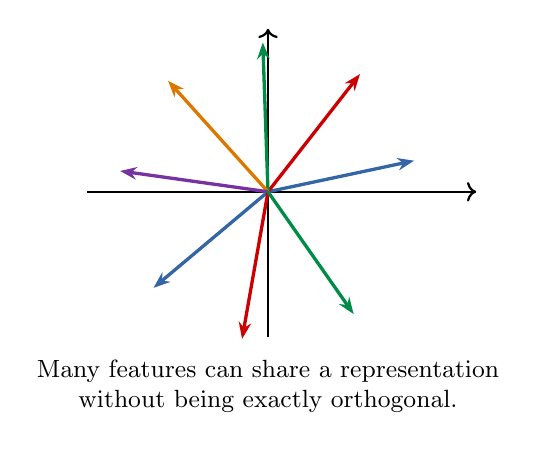
\begin{tikzpicture}[scale=1.15]
\draw[->,thick] (-2,0)--(2.3,0);\draw[->,thick] (0,-1.6)--(0,1.8);
\foreach \a/\c in {12/popblue,52/sampred,92/paramgreen,132/orange1,172/violet1,220/popblue,260/sampred,305/paramgreen}{\draw[-{Stealth[length=6pt]},very thick,\c] (0,0)--({1.65*cos(\a)},{1.65*sin(\a)});}
\node[font=\small,align=center] at (0,-2.15) {Many features can share a representation\\without being exactly orthogonal.};
\end{tikzpicture}
\end{center}
\column{0.52\textwidth}
\begin{itemize}\setlength\itemsep{0.55em}
\item A single activation dimension may help encode several features.
\item In high dimensions, many directions can have small pairwise overlap.
\item The price is polysemanticity: one neuron can respond to different concepts in different contexts.
\end{itemize}
\end{columns}
\vfill\small Elhage et al. (2022), \textit{Toy Models of Superposition}.
\end{frame}

\begin{frame}
\frametitle{Why near-right angles matter}
\begin{center}
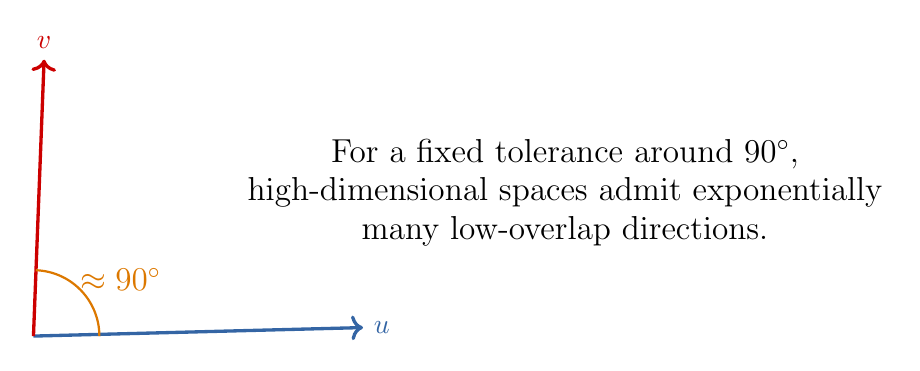
\begin{tikzpicture}[scale=1.35]
\draw[->,very thick,popblue] (0,0)--(3.1,.08) node[right] {$u$};
\draw[->,very thick,sampred] (0,0)--(.1,2.6) node[above] {$v$};
\draw[orange1,thick] (.62,0) arc[start angle=0,end angle=88,radius=.62];
\node[orange1,font=\large\bfseries] at (.82,.53) {$\approx90^\circ$};
\node[align=center,font=\large] at (5.0,1.35) {For a fixed tolerance around $90^\circ$,\\high-dimensional spaces admit exponentially\\many low-overlap directions.};
\end{tikzpicture}
\end{center}
\vfill\small Nearly orthogonal does not mean independent. It means interference can be small enough for sparse features to coexist.
\end{frame}

\begin{frame}
\frametitle{Response: sparse autoencoders recover feature-like directions}
\begin{center}
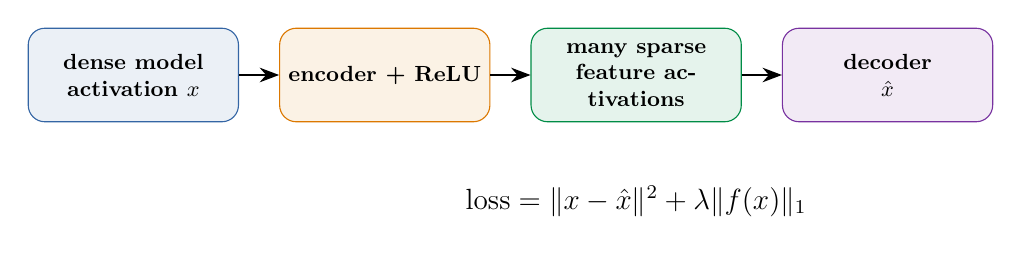
\begin{tikzpicture}[node distance=.55cm and .58cm,scale=.88,transform shape]
\node[draw=popblue,fill=popblue!10,rounded corners=6pt,text width=2.8cm,minimum height=1.35cm,align=center,font=\small\bfseries] (act) {dense model\\activation $x$};
\node[draw=orange1,fill=orange1!10,rounded corners=6pt,text width=2.8cm,minimum height=1.35cm,align=center,font=\small\bfseries,right=of act] (enc) {encoder + ReLU};
\node[draw=paramgreen,fill=paramgreen!10,rounded corners=6pt,text width=2.8cm,minimum height=1.35cm,align=center,font=\small\bfseries,right=of enc] (feat) {many sparse\\feature activations};
\node[draw=violet1,fill=violet1!10,rounded corners=6pt,text width=2.8cm,minimum height=1.35cm,align=center,font=\small\bfseries,right=of feat] (dec) {decoder\\$\hat{x}$};
\foreach \a/\b in {act/enc,enc/feat,feat/dec} \draw[-{Stealth[length=7pt]},thick] (\a)--(\b);
\node[below=.8cm of feat,align=center,font=\large] {$\text{loss}=\|x-\hat{x}\|^2+\lambda\|f(x)\|_1$};
\end{tikzpicture}
\end{center}
\vfill\small If individual neurons are polysemantic, a sparse feature dictionary gives a more useful unit of interpretation. Bricken et al. (2023) reconstruct activations while encouraging only a few active features.
\end{frame}

% ----------------------------------------------------------------
\section{Takeaways}
\transition{Takeaways}{Interpretability asks for mechanisms, not just visual patterns.}

\begin{frame}
\frametitle{Recap}
\begin{enumerate}\setlength\itemsep{0.47em}
\item Grokking separates fast memorization from delayed generalization.
\item A transformer moves addend information into the $=$ residual stream, transforms it through an MLP, then reads answer logits.
\item Fourier pairs make modular addition geometrically simple: adding residues is adding phases.
\item A real explanation requires causal tests, then richer feature tools for larger models.
\end{enumerate}
\vfill
\begin{center}\fcolorbox{paramgreen}{paramgreen!8}{\parbox{0.84\linewidth}{\centering\large\textbf{Question to carry forward:} Which internal directions are necessary for the model's answer?}}\end{center}
\end{frame}

\begin{frame}
\frametitle{Sources and visual credits}
\small
\begin{itemize}\setlength\itemsep{0.40em}
\item Power et al. (2022), \textit{Grokking: Generalization Beyond Overfitting on Small Algorithmic Datasets}.
\item Nanda et al. (2023), \textit{Progress Measures for Grokking via Mechanistic Interpretability}.
\item Gurnee et al. (2025), \textit{When Models Manipulate Manifolds: The Geometry of a Counting Task}.
\item Bricken et al. (2023), \textit{Towards Monosemanticity: Decomposing Language Models With Dictionary Learning}.
\item Elhage et al. (2022), \textit{Toy Models of Superposition}.
\item Welch Labs video stills: \textit{The most complex model we actually understand}, 2025.
\end{itemize}
\end{frame}

\end{document}

% Provenance:
% - Selected Welch Labs frames are full-slide background frames with a small attribution overlay.
% - No local training-run figures are used.
% - Native explanatory figures are pedagogical, based on the cited primary papers.
